\documentclass{article}
\usepackage{graphicx} % Required for inserting images
\usepackage[margin=1in]{geometry}
\usepackage{amsmath}
\usepackage{amsfonts}
\usepackage{amsthm}
\usepackage{thm-restate}
\usepackage[]{hyperref}
\usepackage{cleveref}
\usepackage[dvipsnames]{xcolor}
\usepackage{bbm}
\usepackage{dirtytalk}
\usepackage{graphicx}
\usepackage{subcaption}
\usepackage{float}
\usepackage{tikz}
\usepackage{algorithm}
\usepackage[noend]{algpseudocode}
\usetikzlibrary{arrows.meta,decorations.markings, calc, positioning}


\declaretheorem[name=Theorem,numberwithin=section]{thm}
\declaretheorem[name=Lemma,numberwithin=section]{lemma}
\declaretheorem[name=Assumption,numberwithin=section]{asmpt}
\declaretheorem[name=Proposition,numberwithin=section]{prop}
\declaretheorem[name=Corollary,numberwithin=section]{corollary}
\declaretheorem[name=Remark,numberwithin=section]{rmk}
\declaretheorem[name=Definition,numberwithin=section]{defn}

\newcommand{\man}{\mathcal{M}}
\DeclareMathOperator{\esssup}{esssup}
\definecolor{cyan}{cmyk}{1, 0.4, 0, 0} 
\newcommand{\ndfg}[1]{{\color{magenta}[Florian: #1]}}
\newcommand{\tls}[1]{{\color{cyan}[TLS: #1]}}
\newcommand{\pac}{\mathcal{P}_{2, \text{ac}}(\mathbb{R}^d)}
\newcommand{\posm}{\mathfrak{M}_+(\mathbb{R}^d)}

\usepackage[numbers]{natbib}
\bibliographystyle{unsrtnat}

\title{Hellinger Kantorovich Parallel Transport for Counterfactual Dynamics Estimation}
\author{Florian Gunsilius, Gonzalo Mena, Tristan Saidi, Larry Wasserman}

\begin{document}

\maketitle


\section{Introduction}

\section{Wasserstein and HK Spaces}

In this section we describe the construction of Wasserstein space and its pseudo-Riemannian properties.  We will then use this construction to define an analogous space corresponding to general positive measures instead of probability measures based on the principles of unbalanced transport. This construction follows closely the construction described in \cite{clancy2021interpolating, chewi2024statisticaloptimaltransport, liero2018optimal, liero2016optimal, chizat2018interpolating, kondratyev2016newoptimaltransportdistance}.  

\subsection{Optimal Transport} \tls{Need to revisit these definitions with the tangent cone construction}
Define $\mathcal{P}_{2}(\man)$ to be the set of probability measures over a Riemannian manifold $\man$ with metric tensor $g$ with finite $2^{\text{nd}}$ moment. The $2$-Wasserstein distance between two probability measures $\mu, \nu \in \mathcal{P}_{2}(\mathbb{R}^d)$ is defined by
\begin{equation}
    W_2(\mu, \nu) = \inf_{\gamma \in \Gamma_{\mu, \nu}}\left(\int d_{\man}(x,y)^2\gamma(dx, dy)\right)^{1/2} \label{eq: 2 wasserstein dist}
\end{equation}
where $\Gamma_{\mu, \nu}$ denotes the set of couplings of $\mu$ and $\nu$. The $2$-Wasserstein distance (which we will henceforth refer to as the Wasserstein distance) is indeed a metric, which renders $(\mathcal{P}_{2}(\man), W_2)$ a metric space. A key result is that of Brenier, who showed that the optimal coupling takes the form $(X, \nabla \varphi(X)), X \sim \mu$ for some convex $\varphi$ when $\mu$ is absolutely continuous with respect to the Lebesgue measure.

\begin{restatable}[Brenier]{thm}{}
    Let $\mu, \nu \in \mathcal{P}_2(\mathbb{R}^d)$ be probability measures such that $\mu$ has a density, and let $X \sim \mu$. If $\gamma^*$ is optimal for \cref{eq: 2 wasserstein dist} with $\man = \mathbb{R}^d$, then there exists a convex function $\varphi:\mathbb{R}^d \rightarrow \mathbb{R}$ such that $(X, \nabla\varphi(X))\sim \gamma^*$. 
\end{restatable}

This theorem guarantees that if the source measure has a density, then the optimal transport coupling can be written as the source measure $\mu$ and $\nabla \varphi_\#\mu$, the pushforward of the source under some convex function. The function $\nabla\varphi$ is often referred to as the \textit{Brenier map}. This key theorem will be central to our construction of pseudo-Riemannian structure on the space of probability measures. 

\subsection{Dynamic Formulation and Unbalanced Transport}

Now we'll define $\mathcal{P}_{2}(\man)$ to be the set of probability measures over $\man$ with finite second moment. Let $(v_t)_{t \geq 0}$ be a time dependent family of vector fields over $\man$, and consider the ODE $\dot X_t = v_t(X_t)$. Let $\mu_t$ denote the law of $X_t$, where $X_0 \sim \mu_0$ and $X_t$ evolves according to the ODE described previously. Then, the dynamics of $\mu_t$ obey the so-called \textit{continuity equation},
\begin{equation}
    \partial_t\mu_t + \nabla \cdot (\mu_t v_t) = 0 \label{eq: balanced continuity eqn}
\end{equation}
in the weak sense. It turns out, one can identify optimal transport maps with vector fields satisfying the continuity equation that are optimal in a certain sense. This gives rise to the \textit{dynamic} formulation of optimal transport.

\begin{restatable}[Benamou-Brenier]{thm}{}
    Let $\mu_0, \mu_1 \in \mathcal{P}_{2}(\man)$. Then 
    \begin{equation*}
        W_2(\mu_0, \mu_1) = \inf \left\{\left(\int_{0}^1\|v_t\|^2_{L_2(\mu_t)} dt\right)^{1/2} \, \Bigg| \, (\mu_t, v_t) \text{ solves \cref{eq: balanced continuity eqn}}\right\}.
    \end{equation*}
    Moreover, when $\man = \mathbb{R}^d$ and $\mu_0, \mu_1$ have densities, then the optimal curve $(\mu_t)_{t\geq 0}$ is unique and is described by $X_t \sim \mu_t$, where $X_t = (1-t)X_0 + tX_1$ and $(X_0, X_1) \sim \gamma^* \in \Gamma_{\mu_0, \mu_1}$ with $\gamma^*$ being an optimal coupling.
\end{restatable}

This dynamical formulation, which considers minimum cost transport between probability measures, can be augmented to allow for \textit{unbalanced} transport -- transport where the source and target measures do not necessarily have total mass $1$. To do this, we can create a modified continuity equation that allows for the creation and destruction of mass,
\begin{equation}
    \partial_t\mu_t + \nabla \cdot (\mu_tv_t) = 4\alpha_t\mu_t. \label{eq: unbalanced continuity eqn}
\end{equation}
This leads to an analogous notion of distance between general non-negative measures, commonly referred to as the \textit{Wasserstein-Fisher-Rao} (WFR) or the \textit{Hellinger-Kantorovich} (HK) distance. In fact, in \citet{liero2018optimal} it was shown that HK is indeed a metric on the space of non-negative measures over $\mathbb{R}^d$. 

\begin{restatable}[Hellinger-Kantorovich Distance]{defn}{}
    Let $\mathfrak{M}_+(\mathbb{R}^d)$ denote the space of non-negative measures on $\mathbb{R}^d$. For any $\mu_0, \mu_1 \in \mathfrak{M}_+(\mathbb{R}^d)$ we define the Hellinger-Kantorovich distance to be
    \begin{equation}
        \text{HK}(\mu_0, \mu_1) = \inf\left\{\left(\int_0^1 \left(\|v_t\|_{L_2(\mu_t)}^2 + |\alpha_t|_{L_2(\mu_t)}^2\right)dt\right)^{1/2} \, \Bigg| \, (\mu_t, v_t,  \alpha_t) \text{ solves \cref{eq: unbalanced continuity eqn}}\right\}.
    \end{equation}
\end{restatable}

\subsection{Riemannian structure of $(\mathcal{P}_{2}(\man), W_2)$ and $(\mathfrak{M}_+(\mathbb{R}^d), \text{HK})$}

\textbf{The Tangent Space}. We are almost in a position to describe the Riemannian-like structure of $(\mathcal{P}_{2, \text{ac}}(\man), W_2)$ and $(\mathfrak{M}_+(\mathbb{R}^d), \text{HK})$. But first, we will define a notion of a \say{derivative} in a general metric space.

\begin{restatable}[Metric Derivative]{defn}{}
    Let $(\mathcal{X}, d)$ be a metric space and $(x_t)_{t \geq 0}$ be a curve in $\mathcal{X}$. The metric derivative of the curve at time $t$ is given by
    \begin{equation*}
        |\dot x|(t) := \lim_{s\rightarrow t}\frac{d(x_s, x_t)}{|s - t|}
    \end{equation*}
    provided that the limit exists. 
\end{restatable}

Now, for a pair of probability measures $\mu, \nu \in \mathcal{P}_{2, \text{ac}}(\mathbb{R}^d)$ where $\mu$ admits a density, we will write $T_{\mu \rightarrow \nu}$ for the Brenier map from $\mu$ to $\nu$ and we will write $|\dot \mu|$ for the metric derivative of a curve in $\mathcal{P}_{2, \text{ac}}(\mathbb{R}^d)$ with respect to the Wasserstein metric.

\begin{restatable}[\citet{chewi2024statisticaloptimaltransport}]{thm}{}
    Let $(\mu_t)_{t\geq 0}$ be a regular curve, i.e. $\mu_t$ admits a density and $|\dot \mu_t|$ exists for all $t \geq 0$. Then for every family of vector fields $(v_t)_{t\geq 0}$ for which \cref{eq: balanced continuity eqn} holds, it holds that $|\dot \mu_t|(t) \leq \|v_t\|_{L_2(\mu_t)}$ for all $t \geq 0$. Moreover, there exists a unique family $(v_t)_{t\geq 0}$ such that \cref{eq: balanced continuity eqn} holds and for which $|\dot \mu_t|(t) = \|v_t\|_{L_2(\mu_t)}$ for every $t \geq 0$. This family is such that
    \begin{equation*}
        v_t = \lim_{h \rightarrow0^+}\frac{T_{\mu_t\rightarrow \mu_{t+h}}- I_d}{h} \qquad \text{ in $L_2(\mu_t)$}
    \end{equation*}
    where $I_d$ is the identity map. It also holds that 
    \begin{equation*}
        v_t = \min \left\{\|\tilde{v}_t\|_{L_2(\mu_t)}^2 \, \Big|\, \partial_t\mu_t + \nabla \cdot (\tilde v_t\mu_t) = 0\right\}.
    \end{equation*}
\end{restatable}

Note that Brenier's theorem indicates that the velocity field that coincides (in an $L_2(\mu_t)$ sense) with the metric derivative is a limit of gradients -- in particular, $(T_{\mu_t \rightarrow \mu_{t+h}} - I_d)(x) = \nabla (\varphi(x) - \frac{1}{2}\|x\|_2^2)$. This key fact gives rise to an intuitive definition of the tangent space and a metric tensor for $(\mathcal{P}_{2, \text{ac}}(\mathbb{R}^d), W_2)$ at a measure $\mu$. 

\begin{restatable}[Wasserstein Tangent Space]{defn}{}
    Let $\mu \in \mathcal{P}_2(\man)$. We define the tangent space to $\mathcal{P}_2(\man)$ at $\mu$ to be 
    \begin{equation}
        T_\mu \mathcal{P}_2(\man) = \overline{\left\{\nabla \psi \, | \, \psi \in \mathcal{C}_c^{\infty}\right\}}^{L_2(\mu)}
    \end{equation}
    where $\overline{\{\cdot \}}^{L_2(\mu)}$ denotes the $L_2(\mu)$ closure and $\mathcal{C}_c^{\infty}$ denotes the set of compactly supported and smooth maps. We also endow $T_\mu \mathcal{P}_2(\man)$ with the metric tensor
    \begin{equation}
        \langle \nabla \psi_1, \nabla \psi_2\rangle_{\mu} = \int \langle\nabla\psi_1, \nabla\psi_2 \rangle_g d\mu. 
    \end{equation}
\end{restatable}
We are now in a position to define analogous structure on the Hellinger Kantorovich space, $(\posm, \text{HK})$. Starting from the augmented continuity equation, one can show that the minimum norm solution is unique and is the gradient of a potential. We can then use this to construct the tangent space and the metric tensor as we did for the Wasserstein space.
\begin{restatable}[\citet{clancy2021interpolating}]{prop}{}
    For $\man = \mathbb{R}^d$, we have
    \begin{equation*}
        (v_t, \alpha_t) = \min\left\{\|\tilde v_t\|_{L_2(\mu_t)^2} + |\tilde \alpha_t|_{L_2(\mu_t)^2  }  \, \Big| \, \partial_t\mu_t + \nabla \cdot (\tilde v_t \mu_t) = 4\tilde \alpha_t \mu_t\right\}
    \end{equation*}
    with $(v_t, \alpha_t) \in \overline{\left\{(\nabla \varphi, \varphi) \, | \, \varphi \in \mathcal{C}^{\infty}_{c}\right\}}^{L_2(\mu_t)}$.
\end{restatable}
\begin{restatable}[Hellinger-Kantorovich Tangent Space]{defn}{}
    Let $\mu \in \posm$. We define the tangent space to $\posm$ at $\mu$ to be 
    \begin{equation}
        T_\mu \posm = \overline{\left\{(\nabla \varphi, \varphi) \, | \, \varphi \in \mathcal{C}_c^{\infty}\right\}}^{L_2(\mu)}.
    \end{equation}
    We also endow $T_\mu \posm$ with the metric tensor
    \begin{equation}
        \langle s_1,  s_2\rangle_{\mu} = \int \left(\langle\nabla\varphi_1, \nabla\varphi_2\rangle + 4\varphi_1\varphi_2 \right) d\mu
    \end{equation}
    for any $s_1, s_2\in T_\mu \posm$, with $s_i = (\nabla \varphi_i, \varphi_i)$ and $\varphi_i \in \mathcal{C}_c^\infty$. 
\end{restatable}

\noindent \textbf{The Covariant Derivative.} 
On an abstract manifold $(\man, g)$ that isn't embedded in an ambient space, we have no obvious way to compare vectors in the tangent space at two points $p, q \in \man$, $p \neq q$. Therefore, we need a way of connecting the separate vector spaces $T_p\man$ and $T_q\man$ when $p \neq q$. One can achieve this by defining a rule $\nabla$ for differentiating vector fields against each other on $\man$ in a way that preserves the structure of the metric $g$.

\begin{restatable}[The Covariant Derivative, \citet{petersen2006riemannian}]{defn}{}
    For a manifold $(\man, g)$ we define the covariant derivative $\nabla$ to be a rule that assigns to each pair of vector fields $X$, $Y$ over $\man$ another vector field $\nabla_XY$ satisfying 
    \begin{enumerate}
        \item \textit{Linearity:} $\nabla_{aX+bZ}Y = a\nabla_XY + b\nabla_ZY.$
        \item \textit{Leibniz/derivation property:} for $f \in C^{\infty}(\man)$ we have $\nabla_X(fY) = X(f)Y + f\nabla_XY$, where $X(f) = g(X, \nabla f)$ is the derivative of $f$ in the direction $X$.
    \end{enumerate}
\end{restatable}

While this gives us a way to connect tangent spaces, the covariant derivative might distort the geometry induced by the metric $g$ -- i.e. it might not be \say{metric compatible}. A fundamental result of Riemannian geometry, however, is that for any Riemannian manifold $(\man, g)$ there exists a \textit{unique} connection that is torsion free and is \say{metric compatible}. 

\begin{restatable}[The fundamental theorem of Riemannian Geometry, \cite{petersen2006riemannian}]{thm}{}
    If $\man$ is endowed with a Riemannian metric $g$, then there exists a unique connection $\nabla$ called the \textit{Levi-Civita connection} that is
    \begin{enumerate}
        \item \textit{Torsion free:} $\nabla_XY - \nabla_YX = [X,Y]$, where $[X,Y]$ is the Lie bracket of $X$ and $Y$. 
        \item \textit{Metric compatible:} $Xg(Y, Z) = g(\nabla_XY, Z) + g(Y, \nabla_XZ).$ 
    \end{enumerate}
\end{restatable}
In the case of $(\pac, W_2)$ and $(\posm, \text{HK})$ we can explicitly construct the covariant derivative, but we need to manually verify that they are torsion free and metric compatible as neither spaces are true Riemannian Manifolds.

\begin{restatable}[Wasserstein Covariant Derivative, \citet{clancy2021interpolating}]{prop}{} \label{Wasserstein covariant deriv}
    Let $(\mu_t)_{t\geq 0}$ be a curve through $\pac$ with tangent field $\nabla \varphi_t$ solving \cref{eq: balanced continuity eqn}, and therefore driving the dynamics of $\mu_t$. Also let $v_t$ be another vector field along $\mu_t$ and let $\Pi_{\mu_t}$ be the orthogonal projection onto $T_{\mu_t}\pac$ in $L_2(\mu_t)$. Then the differential operator $\nabla_{(\nabla\varphi_t)}^{W_2}$ given by
    \begin{equation*}
        \nabla_{(\nabla\varphi_t)}^{W_2}v_t = \Pi_{\mu_t}\left(\partial_t v_t + \nabla v_t \cdot \nabla \varphi_t\right)
    \end{equation*}
    is a valid covariant derivative, is torsion free, and is metric compatible. 
\end{restatable}

\begin{restatable}[Hellinger-Kantorovich Covariant Derivative, \citet{clancy2021interpolating}]{prop}{} \label{HK covariant deriv}
    Let $(\mu_t)_{t\geq 0}$ be a curve through $\posm$ with tangent field $(\nabla \varphi_t, \varphi_t)$ solving \cref{eq: unbalanced continuity eqn}, and therefore driving the dynamics of $\mu_t$. Also let $(v_t, \beta_t)$ be another vector field along $\mu_t$ and let $\Pi_{\mu_t}$ be the orthogonal projection onto $T_{\mu_t}\posm$ in $L_2(\mu_t)$. Then the differential operator $\nabla_{(\nabla\varphi_t, \varphi_t)}^{\text{HK}}$ given by
    \begin{equation*}
        \nabla_{(\nabla\varphi_t, \varphi_t)}^{\text{HK}} \begin{pmatrix}
            v_t \\
            \beta_t
        \end{pmatrix} = \Pi_{\mu_t}\begin{pmatrix}
            \partial_t v_t + \nabla v_t \cdot \nabla \varphi_t + 2\beta_t\nabla\varphi_t \\
            \partial_t \beta_t + \frac{1}{2}\langle \nabla \beta_t, \nabla \varphi_t\rangle + 2\varphi_t\beta_t
        \end{pmatrix}
    \end{equation*}
    is a valid covariant derivative, is torsion free, and is metric compatible. 
\end{restatable}

\noindent \textbf{The Exponential and Logarithmic Maps.} For $\mathcal{P}_{2, \text{ac}}(\man)$, the exponential map is defined to be $\mathbf{exp}_{\mu}(u) := (\exp(u))_\#\mu$ where $\exp(\cdot)$ is the exponential map of $\man$ and $u \in L_2(\mu)$. In the case of $\man = \mathbb{R}^d$, this operation is trivial -- we have
\begin{equation}\label{eq: wasserstein euclidean expmap}
    \mathbf{exp}_\mu(u) = (I_d + u)_\# \mu
\end{equation}
where $I_d$ is the identity map, $x \mapsto x$. In the case of the logarithmic map, things are analogous. We define $(\mathbf{log}_\mu\nu) (x) := \log_x(T_{\mu \rightarrow \nu}(x))$ where $T_{\mu \rightarrow \nu}$ is the Brenier map from $\mu$ to $\nu$. Note that we will denote $\overline{\log}$ as the normalized vector (with respect to the metric tensor). Again, in the Euclidean case this reduces to
\begin{equation}\label{eq: wasserstein euclidean logmap}
    (\mathbf{log}_\mu\nu )(x) = (T_{\mu \rightarrow \nu} - I_d)(x).
\end{equation}


\subsection{Hellinger-Kantorovich Geometry via Cone Lifting}

Amazingly, \citet{liero2016optimal} show that Hellinger-Kantorovich geometry arises from $W_2$ geometry on an augmented base domain. In particular, this construction entails lifting positive measures on the base space $\man$ to probability measures on $\mathfrak{C}(\man)$, the metric cone of the base space ($\man$). Under a particular set of lifts, it turns out that the Wasserstein geometry on the cone is identical to the Hellinger-Kantorovich geometry on the original space.

\subsubsection{Metric Cones}

\begin{restatable}[Metric cone, \citet{burago2001course}]{defn}{} \label{def: metric cone}
    For a Riemannian manifold $(\man, g)$, the metric cone is
    \[\mathfrak{C}_\man = \man \times \mathbb{R}_{+} / \{(x, 0) \sim (y, 0)\}\]
    where a point in $\mathfrak{C}_\man$ is written as $(x, r)$. The metric tensor on the cone is given by $g_{(x,r)} = dr^2 + r^2g_x$, while the metric (as one would have in a metric space) is given by 
    \begin{equation*}
    d_{\mathfrak{C}}(z_0, z_1)^2 = r_0^2 + r_1^2 - 2r_0r_1\cos(d_{\man}(x_0, x_1) \land \pi)
    \end{equation*}
    for $z_i = (x_i, r_i)$.
\end{restatable} 

For metric cones of Euclidean space, we are fortunate in the sense that geodesics are available in closed form. This is made explicit and precise below.

\begin{restatable}[Geodesics on $\mathfrak{C}_{\Omega}$, $\Omega \subset\subset  \mathbb{R}^d$, \citet{liero2016optimal}]{prop}{}
    The function $Z(s; \cdot, \cdot ):\mathfrak{C}_\Omega \times \mathfrak{C}_\Omega \rightarrow \mathfrak{C}_\Omega$ given by 
    \begin{equation} \label{eq: cone geodesics}
        Z(s; z_0, z_1) = \left[X\left(s; z_0, z_1\right) , R\left(s; z_0, z_1\right)\right]
    \end{equation}
    where
    \begin{align*}
        R(s; z_0, z_1)^2 &= (1-s)^2r_0^2 + s^2r_1^2 + 2s(1-s)r_0r_1\cos(\min\{\pi, \|x_0 - x_1\|_2\}) \\
        \\[0.25ex]X(s; z_0, z_1) &= (1 - \rho(s; z_0, z_1))x_0 + \rho(s; z_0, z_1)x_1 \\
        \\[0.05ex]\rho(s; z_0, z_1) &= \begin{cases}
            \frac{1}{\|x_0 - x_1\|_2}\arccos\left(\frac{(1-s)r_0 + sr_1\cos(\|x_0 - x_1\|_2)}{R(s; z_0, z_1)}\right) & \text{for }\|x_0 - x_1\|_2 < \pi \\
            \frac{1}{2}\left(1 + \text{sign}((1-s)r_0 + sr_1)\right) & \text{otherwise}
        \end{cases}
    \end{align*}
    is a unique constant-speed geodesic between $z_0$ and $z_1$ where $d_{\mathfrak{C}}(\gamma(s), \gamma(t)) = |t-s|d_{\mathfrak{C}}(z_0, z_1)$. 
\end{restatable}

From this closed form expression, we can directly compute the exponential and logarithmic map on $\mathfrak{C}_\Omega$, the proof for which we provide in \Cref{sec: proof of main results}.
\begin{restatable}[Exponential and Logarithmic maps on $\mathfrak{C}_\Omega$]{prop}{} \label{cone exponential and log map}
    Let $z_i = (x_i, r_i) \in \mathfrak{C}_{\Omega}$ and let $(v_x, v_r) \in T_{z_0}\mathfrak{C}_\Omega$ with $\|v_x\|_2 > 0$. Then for $0 < \|x_0 - x_1\|_2 < \pi$ we have
    \begin{equation} \label{eq: cone exp map}
        \exp^{\mathfrak{C}}_{z_0}((v_x, v_r)) = \left(x_1, r_1\right)
    \end{equation}
    with 
    \begin{equation*}
        x_1 = x_0 + \theta\frac{v_x}{\|v_x\|_2}, \quad r_1 = \sqrt{\|v_x\|_2^2r_0 + (v_r+r_0)^2}, \quad \theta = \text{atan2}(r_0\|v_x\|_2, v_r + r_0)
    \end{equation*}
    and 
    \begin{equation} \label{eq: cone log map}
        \log_{z_1}^\mathfrak{C}(z_0) = \left[\frac{\sin(\|x_1 - x_0\|_2)r_1}{\|x_1 - x_0\|_2r_0}, r_1\cos(\|x_1 - x_0\|_2) - r_0\right].
    \end{equation}
\end{restatable} 

\subsubsection{Lifting Measures, Geodesics and Tangent Vectors on $\mathfrak{M}_+(\man)$ to $\mathcal{P}_{2}(\mathfrak{C}_\man)$.}
Now, given a measure $\lambda \in \mathfrak{M}(\mathfrak{C}_{\man})$ we can project it to a measure in $\mathfrak{M}(\man)$ with the map $\mathfrak{B}$ defined as,
\begin{equation} \label{eq: measure projection}
    \int_{\man} \phi(x)d\mathfrak{B}\lambda(x) = \int_\man r^2 \phi(x) d\lambda(x, r) \qquad \text{for all test functions }\phi \in C^0(\man).
\end{equation}
Clearly, there are many possible ways to define a lift of a measure. In fact, any $\lambda$ of the form
\begin{equation*}
    \lambda(dx, dr) = \eta(x, dr)\mathfrak{B}\lambda(dx) \qquad \text{with } \qquad \int_0^\infty r^2\eta(x, dr) = 1 \text{ \quad for $\mathfrak{B}\lambda$ a.e. $x$}
\end{equation*}
will do. However, \citet{liero2016optimal} show that one can replicate Hellinger-Kantorovich geometry on some base space $\man$ through Wasserstein geometry on the cone space $\mathfrak{C}_\man$ by minimizing over all possible lifts.

\begin{restatable}[Wasserstein distance on $\mathfrak{C}_\man$]{defn}{} \label{def: cone wasserstein}
    Let $\lambda_1, \lambda_2 \in \mathfrak{M}(\mathfrak{C}_\man)$ and suppose that $\lambda_1(\mathfrak{C}_\man) = \lambda_2(\mathfrak{C}_\man)$. Then we set
    \begin{equation*}
        W_{\mathfrak{C}}(\lambda_0, \lambda_1) = \inf \left\{\int_{\mathfrak{C}_{\Omega}\times\mathfrak{C}_{\Omega}}d_{\mathfrak{C}}(z_0, z_1)^2 \gamma(dz_0, dz_1) \,\bigg|\,  \gamma \in \mathfrak{M}(\mathfrak{C}_{\Omega}\times\mathfrak{C}_{\Omega}), \,\Pi^i_{\#}\gamma = \lambda_i\right\}.
    \end{equation*}
\end{restatable}
Under this definition of Wasserstein geometry on $\mathfrak{C}_\man$, we have the following Theorem.

\begin{restatable}[Equivalence of $(\mathcal{P}(\mathfrak{C}_\man), W_2)$ and $(\mathfrak{M}_+(\man), \text{HK})$, \citet{liero2016optimal} Theorem 3.6]{thm}{}
    For any measures $\mu_0, \mu_1 \in \mathfrak{M}_+(\man)$ we have 
    \begin{equation} \label{eq: cone wasserstein and hk equivalence}
    \text{HK}(\mu_0, \mu_1) = \min\left\{W_{\mathfrak{C}}(\lambda_0, \lambda_1) \,\Big|\, \lambda_i \in \mathcal{P}(\mathfrak{C}_\man),  \mathfrak{B}\lambda_0 = \mu_0, \mathfrak{B}\lambda_1 = \mu_1\right\}.
\end{equation}
\end{restatable}
This incredible result allows us to leverage key aspects of Wasserstein geometry when analyzing and understanding the geometry of the unbalanced Hellinger-Kantorovich space. This connection will be a key aspect of our approach. But before describing how we will leverage this result, we need to address a significant challenge -- minimizing over all such lifts in \cref{eq: cone wasserstein and hk equivalence} is not computationally tractable. Fortunately, one can leverage \textit{another} equivalent formulation of the Hellinger-Kantorovich distance to obtain explicit lifts that are optimal in the sense of \cref{eq: cone wasserstein and hk equivalence}.
\\

\noindent \textbf{The Logarithmic Entropy Transport Functional.}
To compute the Hellinger-Kantorovich distance and a pair of optimal lifts we will use an equivalent characterization. Let $\eta_j = \Pi^j_\#\eta$ and define the Hellinger-Kantorovich entropy-transport functional as
\begin{equation} \label{eq: let functional}
    E(\eta; \mu_0, \mu_1) = \int_{\man}F\left(\frac{d\eta_0}{d\mu_0}\right)d\mu_0 + \int_{\mathbb{\man}}F\left(\frac{d\eta_1}{d\mu_1}\right)d\mu_1 + \int_{\man \times \man}c(d_{\man}(x_0, x_1))d\eta
\end{equation}
where
\begin{equation*}
    c(L) = \begin{cases}
        -2\log(\cos(L)) & L < \pi/2 \\
        \infty & L \geq \pi/2
    \end{cases}
\end{equation*}
and $F(\rho) = \rho\log\rho - \rho + 1.$ \citet{liero2016optimal} show that 
\begin{align} \label{eq: let hk equivalence}
    \text{HK}(\mu_0, \mu_1) &= \inf\left\{E(\eta;\mu_0, \mu_1)^{1/2} \, |\, \eta  \in \mathfrak{M}(\man \times \man), \eta_j  \ll \mu_j\right\}.
\end{align}
They also show that the logarithmic entropy transport functional gives us a way to compute optimal lifts in the sense of \cref{eq: cone wasserstein and hk equivalence}. In particular, assume that $\eta \in \mathfrak{M}(\man \times \man)$ is a minimizer of $E(\cdot\,; \mu_0, \mu_1)$ and for the marginals $\eta_i$ consider the Lebesgue decomposition $\mu_i = \sigma_i\eta_i + \mu_i^\perp$. Then the transport plan $\gamma_{\eta} \in \mathfrak{M}(\mathfrak{C}_{\man} \times \mathfrak{C}_{\man})$ defined by
\begin{multline}\label{eq: optimal lift}
    \gamma_{\eta}(dz_0, dz_1) = \delta_{\sqrt{\sigma_0(x_0)}}(dr_0)\delta_{\sqrt{\sigma_1(x_1)}}(dr_1)\eta(dx_0, dx_1) \\
    + \delta_1(dr_0)\mu_0^\perp(dx_0)\delta_{\mathfrak{o}}(dz_1) + \delta_1(dr_1)\mu_1^\perp(dx_1)\delta_{\mathfrak{o}}(dz_0) 
\end{multline}
and the associated lifts $\lambda_i = \Pi_{\#}^i\gamma_\eta$ are optimal for \cref{eq: cone wasserstein and hk equivalence}. This means we can solve the logarithmic-entropy-transport functional approach and use the optimal plan to construct appropriate lifts of the original measures onto the cone. 


\begin{algorithm}[H]
    \begin{algorithmic}[1] \label{alg: lift measures to cone}
        \caption{Lift measures from  $(\mathfrak{M}_+(\mathbb{\man}), \text{HK})$ to $(\mathcal{P}_{2, \text{ac}}(\mathfrak{C}_\man), W_2)$}
        \label{alg: let lift}
        \Require Base Riemannian manifold $(\man, g)$, measures $\mu_0, \mu_1 \in \mathfrak{M}_+(\man)$.  
        \State Solve logarithmic entropy transport functional minimization,
        \begin{align*} 
            \text{HK}(\mu, \nu) &= \inf\left\{E(\eta;\mu, \nu)^{1/2} \, |\, \eta  \in \mathfrak{M}(\man \times \man), \,\Pi^1_{\#}\eta  \ll \mu, \, \Pi^2_{\#}\eta \ll \nu\right\} \quad \text{for $E$ defined in \cref{eq: let functional}}
        \end{align*}
        and let $\eta^*$ denote the optimal coupling for the problem above. 
        \State Compute the Lebesgue decompositions $\mu_i = \sigma_i\eta_i + \mu_i^\perp$.
        \State Lift $\mu_i$ to $\lambda_i$ via $\lambda_i = \Pi^i_{\#}\gamma_{\eta}$ with $\gamma_{\eta}$ defined in \cref{eq: optimal lift}.
        \State \Return $\lambda_0, \lambda_1  \in \mathcal{P}_{2, \text{ac}}(\mathfrak{C}_{\man})$. 
    \end{algorithmic}
\end{algorithm}

\noindent \textbf{Geodesic Projections.} Note that these results indicate that optimal lifts are dependent on the source and target measures $\mu_0, \mu_1 \in \mathfrak{M}_+(\man)$ -- this indicates that we need to use caution when constructing algorithms on $\mathfrak{C}_\man$ to emulate Hellinger-Kantorovich geometry on $\man$. Fortunately, it holds that for a pair $\mu_0, \mu_1$, the $W_\mathfrak{C}$ geodesic between optimal lifts $\lambda_0, \lambda_1$ of $\mu_0, \mu_1$ projects back to a Hellinger-Kantorovich geodesic on $\Omega$. 

\begin{restatable}[\citet{liero2016optimal}, Corollary 4.4]{prop}{} \label{cone geodesics project to hk geodesics}
    For any optimal lift $\lambda_0, \lambda_1$ of $\mu_0, \mu_1$, an optimal plan $\gamma \in \mathcal{P}_2(\mathfrak{C}_\Omega \times \mathfrak{C}_\Omega)$ in the sense of \cref{def: cone wasserstein} induces a geodesic path in $(\mathfrak{M}_+(\Omega), \text{HK})$ connecting $\mu_0$ and $\mu_1$ given by
    \[\mu(s) = \mathfrak{B}\lambda(s) \qquad \text{with} \qquad \lambda(s) = Z(s; \cdot, \cdot)_\#\gamma.\]
\end{restatable}
This result indicates that we can interpolate along a Hellinger-Kantorovich geodesic by lifting the source and target measures to $\mathfrak{C}_\man$, solving for the optimal plan, performing Wasserstein interpolation on $\mathfrak{C}_\man$, and projecting back via $\mathfrak{B}$.
\\

\noindent \textbf{Lifting Tangent Vectors.} Fortunately, lifting tangent vectors in a manner that is faithful to the dynamical formulation of Hellinger-Kantorovich geometry is straightforward. This is described in the following result.

\begin{restatable}[\citet{maniglia2007probabilistic}, Proposition 3.6]{prop}{} \label{lifting velocities}
    Let $(v_t)_{t \in [0, T]}$ be a time-varying vector field on $\Omega \subset \subset \mathbb{R}^d$ such that $\|v_t\|_{L_\infty(\Omega)} < \infty$, $\esssup_{x \in \Omega}\|\nabla_xv_t\|_{\text{op}} < \infty$ and 
    \[\int_0^T \left(\|v_t\|_{L_\infty(\Omega)} + \|\nabla_xv_t\|_{\text{op}}\right)dt < \infty.\]
    Further suppose that $\beta_t: [0, T] \times \Omega \rightarrow \mathbb{R}$ is continuous jointly in time and space. Then, for any $\mu_0 \in \mathfrak{M}_+(\Omega)$ there exists a unique and weakly continuous solution to \cref{eq: unbalanced continuity eqn} with $\mu(0) = \mu_0$. Moreover, for any lift $\lambda_0 \in \mathcal{P}(\mathfrak{C}_\Omega)$ of $\mu_0$, the curve given by 
    \[\lambda(t) = \left[X(t; \cdot), R(t; \cdot, \cdot)\right]_{\#} \lambda_0\]
    where $t \mapsto \left(X(t;x), R(t; x, r)\right)$ is a solution to the ODE system
    \[\dot X(t; x) = v_t(X(t;x)), \quad \dot R(t; x, r) = 2\beta_t(X(t; x))R(t; x, r)\]
    with initial conditions $X(0; x) = x$ and $R(0; x, r) = r$ is a lift of $\mu(t)$ in the sense that $\mathfrak{B}\lambda(t) = \mu(t)$. 
\end{restatable}
\noindent Thus, given a tangent vector $(v_t, \beta_t)$ we can lift it to a velocity field on the cone with 
\[V_t^*(x, r) = \left(v_t(x), 2\beta_t(x)r\right).\]

\section{Parallel Transport}

\textbf{Exact Parallel Transport via the Covariant Derivative.} Now we are in a position where we can define parallel transport. Intuitively, a vector field along a curve is \say{unchanging} loosely-speaking if its derivative is zero. Thus, in the context of abstract manifolds, we stipulate that a vector field along a curve is the parallel transport of a source vector if its covariant derivative along the curve is zero.
\begin{restatable}[\citet{lee2018introduction}]{defn}{} \label{parallel transport on general manifolds}
    Let $\man$ be a smooth Riemannian manifold. A smooth vector field $X$ along a smooth curve $\gamma$ is said to be parallel along $\gamma$ with respect to the Levi-Civita connection if $\nabla_{\dot \gamma}X \equiv 0$.
\end{restatable}
This characterization now allows us to define parallel transport on $(\pac, W_2)$ and $(\posm, \text{HK})$ using the covariant derivative. Consider a smooth curve $\mu_t$ through $\pac$ indexed by $t \in (0, 1)$ with the tangent field $\nabla \varphi_t$ driving its dynamics. 

\begin{restatable}[Wasserstein Parallel Transport PDE]{prop}{} \label{Wasserstein parallel transport pde}
    A vector field $v_t$ along $\mu_t$ is parallel along $\mu_t$ with respect to $\nabla_{(\nabla\varphi_t)}^{W_2}$ if
    \begin{equation*}
        \boxed{\nabla \cdot \left(\mu_t\left(\partial_t v_t + \nabla v_t \cdot \nabla \varphi_t\right)\right) = 0 \qquad \text{for a.e. $t \in (0,1).$}}
    \end{equation*}
\end{restatable}
\noindent \textit{Proof.} Due to \Cref{parallel transport on general manifolds} and \Cref{Wasserstein covariant deriv} we know that $v_t$ is parallel along $\mu_t$ if $\Pi_{\mu_t}\left(\partial_tv_t + \nabla v_t \cdot \nabla\varphi_t\right) = 0$ for almost every $t \in (0,1).$ This is tantamount to the requirement that $\nabla \cdot \left(\mu_t(\partial_tv_t + \nabla v_t \cdot \nabla\varphi_t)\right) = 0$ since the $L_2(\mu_t)$ projection simply discards the divergence free portion of the vector field. \qed{}

The same approach is directly applicable for the Hellinger-Kantorovich case. Consider a smooth curve $\mu_t$ indexed by $t \in (0,1)$ with velocity field $(\nabla\varphi_t, \varphi_t)$. 

\begin{restatable}[Hellinger-Kantorovich Parallel Transport PDE]{prop}{} \label{HK parallel transport pde}
    A vector field $(v_t, \beta_t)$ along $\mu_t$ is parallel along $\mu_t$ with respect to $\nabla_{(\nabla\varphi_t, \varphi_t)}^{\text{HK}}$ if
    \begin{align*}
        \boxed{\nabla \cdot (\mu_t (\partial_tv_t + \nabla v_t \cdot \nabla \varphi_t + 2\varphi_t v_t + 2g_t \nabla\varphi_t)) = 0 
        \qquad \text{and} \qquad 
        \partial_tg_t + \frac{1}{2}\langle\nabla g_t, \nabla\varphi_t\rangle + 2\varphi_t g_t = 0.}
    \end{align*}
\end{restatable}
\noindent \textit{Proof.} By \Cref{parallel transport on general manifolds} and \Cref{HK covariant deriv}, a vector field $(v_t, \beta_t)$ is parallel along $\mu_t$ if
\begin{align}
    \Pi_{\mu_t}\left(\begin{bmatrix}
        \partial_tv_t + \nabla v_t\cdot \nabla\varphi_t + 2\varphi_tv_t +  2g_t\nabla\varphi_t \\
        \partial_tg_t + \frac{1}{2}\langle\nabla g_t, \nabla\varphi_t\rangle + 2\varphi_t g_t
    \end{bmatrix}\right) = 0 \qquad \text{for a.e. $t \in (0,1).$ }
\end{align}
The orthogonal projection in the HK case is a Helmholtz decomposition of the vectorial portion of the argument (discarding the zero divergence component) and it leaves the mass creation term unchanged. Thus, we are left with the two conditions that we set out to prove. \qed{}
\\

\noindent \textbf{Approximate Parallel Transport.} While \Cref{Wasserstein parallel transport pde} and \Cref{HK parallel transport pde} describe parallel transport along any curve, solving these PDEs in practice may be challenging, especially in high-dimensional settings. To this end, we describe an alternative approximate but tractable approach for computing parallel transport \textit{along geodesics} -- our approach uses parallel transport on the base space of $\mathcal{P}_{2, \text{ac}}(\man)$ for any Riemannian manifold $\man$. Before we describe said approach, we will introduce \textit{Jacobi fields}, which will be central to our method.

Jacobi fields allow us to measure the effect of curvature on a one parameter family of geodesics. A \textit{Jacobi field} is a vector field along a geodesic $\gamma$ capturing the difference between a geodesic and a perturbed geodesic along the parameter of the family. Concretely, let $\gamma_{\tau}$ be a smooth, one-parameter family of geodesics with $\gamma_0 = \gamma$. Then
\begin{equation}
    J(s) = \frac{\partial}{\partial \tau}\gamma_{\tau}(s)\bigg|_{\tau = 0} \in T_{\gamma(s)}\man
\end{equation}
is a Jacobi field, and it describes the infinitesimal behavior of the geodesic family about $\tau = 0$. Jacobi fields satisfy the so-called Jacobi equation
\begin{equation}
    \nabla_{\dot\gamma}\nabla_{\dot\gamma}J(s) + R(J(s), \dot{\gamma}(s))\dot{\gamma}(s) = 0
\end{equation}
where $\nabla$ is the covariant derivative (typically with respect to the Levi-Civita connection) $\dot{\gamma}(s) = d\gamma(s)/ds$, and $R(\cdot, \cdot)$ is the Riemann curvature tensor. A key fact about Jacobi fields is the following, which arises from the properties of the second-order ODE above. 

\begin{restatable}[Existence and Uniqueness of Jacobi Fields, Proposition 10.2 of \citet{lee2018introduction}]{prop}{}
Let $\gamma_p(s) = \exp_p(su)$ be a geodesic through a Riemannian or pseudo-Riemannian manifold $\man$ for some $u \in T_p\man$. Then for every pair of vectors $v, w \in T_p\man$ there is a unique Jacobi field denoted $j_{p, u}(v, w )(s)$ satisfying the initial conditions $j_{p, u}(v, w )(0) = v$ and $\nabla_{\dot \gamma_p}j_{p, u}(v, w)(0) = w$. 
\end{restatable}

Observe that this result indicates that one can also define Jacobi fields along a geodesic by solely specifying their zero and first order initial conditions. Henceforth, we will denote with $J$ a Jacobi field defined by a variation through geodesics, while we will denote with $j$ a Jacobi field defined through initial conditions. With this in mind, we will show that a particular Jacobi field along $\man$ can be used to approximate parallel transport on $\mathcal{P}_{2, \text{ac}}(\man)$. 

\begin{restatable}[Fanning Scheme, Proposition B.3 of \citet{louis2018fanning}]{prop}{} \label{fanning approximation}
    Let $\Omega \subseteq \man$ be a compact subset of $\man$ with injectivity radius lower bounded by $\eta$, and let $\gamma_p(s) = \exp_p(su)$ be a geodesic through $(\man, g)$ with $\gamma_p([0, s]) \subset \Omega$. Further denote $\mathcal{T}_0^s(v)$ as the parallel transport of $v \in T_{p}\man$ from $p = \gamma_p(0)$ to $\gamma_p(s)$. Then there exists an $A \geq 0$ such that for all $s < \frac{\eta}{\|u\|_g}$ we have   
    \[\left\|s^{-1}j_{p, u}(0, v)(s) - \mathcal{T}_0^s(v)\right\|_g \leq As^2\|v\|_g. \]
\end{restatable}

\begin{restatable}[Approximation of $\mathcal{P}_{2}(\man)$ Parallel Transport]{thm}{}\label{parallel transport approx result} 
    Let $(\man, g)$ be a Riemannian manifold, suppose $\mu_t: [0, 1] \rightarrow \mathcal{P}_{2}(\man)$ is a regular curve with velocity field $\nabla \varphi_t$, and assume that $F_s$ is $\mu_t$-essentially invertible, where $F_s(x) = \exp_x(su_t(x))$. Further let $\nu \in \mathcal{P}_{2}(\man)$ be the target measure and assume that there exists a $u_t$ such that $s \rightarrow \nu_s := \left(F_s\right)_\# \mu_t$, $s \in [0, 1]$ traces out a regular geodesic between $\mu_t$ and $\nu$ that has a velocity field $\nabla\psi_s$ with a Lipschitz constant uniformly bounded in $s$ \tls{I think this is actually a strong assumption - my understanding is that it rules out mass splitting and merging in the singular case, which is SUPER STRICT}. For $s$ sufficiently small then it holds that 
    \[w_t^s = \Pi_{\nu_s}\left(s^{-1}j_{\mu_t, u_t}\left(0, \nabla\varphi_t\right)(s) \right)\]
    with
    \[j_{\mu_t, u_t}\left(0, \nabla\varphi_t\right)(s) := \left(x \mapsto j_{x, u_t(x)}\left(0, \nabla\varphi_t(x)\right)(s)\right) \circ F_s^{-1}\]
    approximates $\mathcal{T}_0^s(\nabla \varphi_t)$, the parallel transport of $\nabla\varphi_t$ along the geodesic $\textbf{exp}_{\mu_t}(su_t)$, in the sense that
    \[\|w_t^s - \mathcal{T}_0^s(\nabla\varphi_t)\|_{L_2(\nu_s)} = O(s^2).\]
\end{restatable}

We provide the proof of \Cref{parallel transport approx result} in \Cref{sec: proof of main results}. This result allows us to approximate compute parallel transport of a tangent vector $v$ on $(\mathcal{P}_{2}(\man), W_2)$ \textit{along geodesics} provided that we are able to solve for the Jacobi field $j_{\mu_t, u_t}$ on the base space $\man$. If one takes the base space $\man = \Omega \subset \subset \mathbb{R}^d$, solving the Jacobi field is trivial. If one wants to compute parallel transport for $(\mathfrak{M}_+(\Omega) ,\text{HK})$ then we can solve the logarithmic entropy transport functional problem in \cref{eq: let hk equivalence}, lift our measures to probability measures on $\mathfrak{C}_{\Omega}$, and do \textit{Wasserstein} parallel transport there. In a later section we detail an approach for solving the required Jacobi field on $\mathfrak{C}_{\Omega}$.  

\tls{As Florian said: Wasserstein parallel transport is obtained by pushing the original tangent vector field through the transport map.}
\begin{algorithm}[H]
    \begin{algorithmic}[1]
        \caption{Parallel transport on $(\mathcal{P}_{2}(\mathbb{R}^d), W_2)$}
        \label{alg: W parallel transport}
        \Require Source measure $\mu \in \mathcal{P}_{2, \text{ac}}(\mathbb{R}^d)$, target measure $\nu \in \mathcal{P}_{2, \text{ac}}(\mathbb{R}^d)$, tangent vector $v \in T_{\mu}\mathcal{P}_{2, \text{ac}}(\mathbb{R}^d)$, approximation resolution $n$.  
        \State Compute the Brenier map $T_{\mu \rightarrow \nu}$ and stepsize $s = W_2(\mu, \nu)/n.$
        \State Compute the maps $F_i = (1 - \frac{i}{n})I_d + \frac{i}{n}T_{\mu \rightarrow \nu}$ for $i \in \{0, \dots, n\}$.
        \State Let $v_1 = v$.
        \For{$i = 1$ to $n$}
            \State Compute the interpolated measure $\mu_i = (F_{i-1})_\#\mu$.
            \State Set $j_{(x, \cdot)}(0, v_i(x))(s) = sv_i(x)$, the solution to the Jacobi equation on $\mathbb{R}^d$.
            \State Define the step map $S_i = F_i \circ F_{i -1}^{-1}.$
            \State Compute $v_{i+1} = \Pi_{\mu_{i+1}}\left(s^{-1}j(0, v_i)(s) \circ S_i^{-1}\right) = \Pi_{\mu_{i + 1}}(v_i \circ S_i^{-1})$. 
        \EndFor
        \State \Return $v_{n+1} \in T_\nu \mathcal{P}_{2, \text{ac}}(\mathbb{R}^d)$. 
    \end{algorithmic}
\end{algorithm}

\tls{HK is more complicated, in part because the lifted measures are always singular.}
\begin{algorithm}[H]
    \begin{algorithmic}[1]
        \caption{Parallel transport on $(\mathfrak{M}_+(\Omega), \text{HK})$}
        \label{alg: HK parallel transport}
        \Require Source measure $\mu \in \mathfrak{M}_+(\Omega)$ and target measure $\nu \in \mathfrak{M}_+(\Omega)$ with $\text{diam}(\Omega) < \pi$, tangent vector $(v, \beta) \in T_{\mu}\mathfrak{M}_+(\Omega)$, approximation resolution $n$.  
        \State Compute the optimal lifts $\lambda_{\mu}, \lambda_{\nu} = \text{LiftToCone}(\mu, \nu)$ via \Cref{alg: let lift}.
        \State Compute the optimal coupling $\pi^* \in \mathcal{P}_2(\mathfrak{C}_{\Omega} \times \mathfrak{C}_{\Omega})$ and stepsize $s = W_\mathfrak{C}(\lambda_\mu, \lambda_\nu)/n.$
        \State Compute the maps $F_i = Z_{(\frac{i}{n})}$ for $i \in \{0, \dots, n\}$ where $Z_t(z_0, z_1) = Z(t; z_0, z_1)$.
        \State Compute the interpolated measures $\lambda_i = (F_{i-1})_\#\pi^*$ for $i \in \{1, \dots, n+1\}$.
        \State Lift $(v, \beta)$ to $V^*_1(x,r) = \left(v(x), 2\beta(x)r\right)$. \Comment{\Cref{lifting velocities}}
        \For{$i = 1$ to $n$}
            \State Obtain intermediate coupling $\pi^*_{i} = (F_{i-1}, F_i)_\#\pi^*$
            \State Compute the approximate parallel transport via the barycentric projection of the Jacobi field,
            \[V^*_{i + 1}(z) = \Pi_{\lambda_{i + 1}}\left(s^{-1}\int j_{\left(y, \, \overline{\log}^{\mathfrak{C}}_y(z)\right)}\left(0, V^*_i(y)\right)(s)d\pi_i^*(y \,|\, z)\right)\]
            \tls{barycentric projection not needed under the assumption that the Lipschitz constant of the velocity field is uniformly controlled -- this is a strong assumption}
            \hspace{\algorithmicindent} where $j_{z, u_i(z)}(0, V_i^*(z))(s)$, is the Jacobi field on $\mathfrak{C}_\Omega$ along $\gamma_z(s) = \exp^{\mathfrak{C}}_z(su_i(z))$ governed by 
            \[\nabla_{\dot \gamma_z}\nabla_{\dot \gamma_z} j_{z, u_i(z)}(0, V_i^*(z))(s) + R\left(j_{z, u_i(z)}(0, V_i^*(z))(s), \dot \gamma_z(s)\right)\dot \gamma_z(s) = 0\]
            \hspace{\algorithmicindent}which can be computed via \Cref{alg: jacobi field}.
        \EndFor
        \State \Return $V^*_{n+1} \in L_2(\lambda_\nu)$. 
    \end{algorithmic}
\end{algorithm}
\begin{figure}[t]
\centering
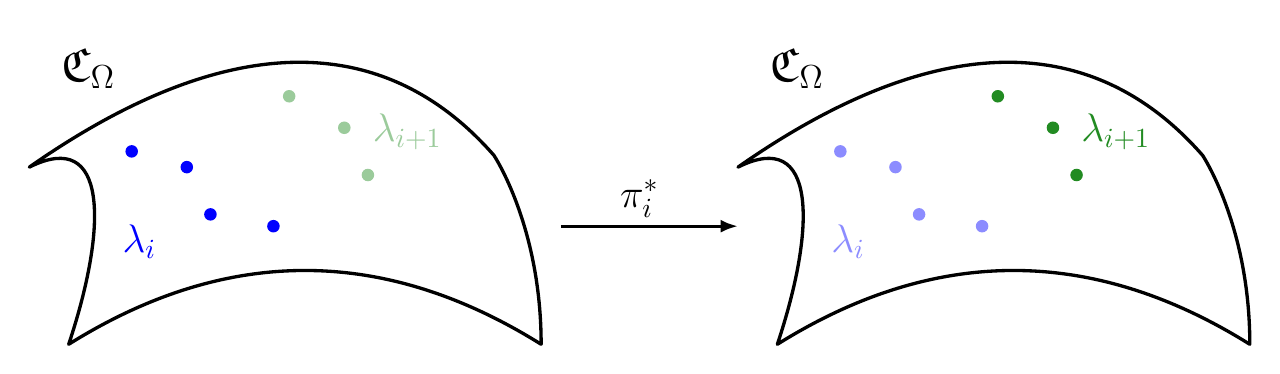
\begin{tikzpicture}[
  scale=1.0,
  >={Latex[length=2.2mm]},
  warp/.style={draw, very thick, line cap=round, line join=round},
  lab/.style={font=\small},
  atom/.style={circle, fill=blue, inner sep=1.6pt},
]

% One warped "square-like" manifold + 4 atoms (Diracs)
\newcommand{\warpsquare}[2]{%
\begin{scope}[xshift=#1cm,yshift=#2cm]
  \draw[warp]
    (-3.5, 0.75)
      .. controls (-1.0, 2.5) and ( 1.0, 2.5) .. ( 2.4, 0.9)
      .. controls ( 2.4, 0.9) and ( 3.0,0.0) .. ( 3.0,-1.5)
      .. controls ( 1.0,-0.25) and (-1.0, -0.25) .. (-3.0,-1.5)
      .. controls (-2.5, 0.0) and (-2.5, 1.25) .. (-3.5, 0.75)
    -- cycle;

  \node[lab] at (-2.75, 2.0) {\LARGE $\mathfrak{C}_\Omega$};
\end{scope}
}

% Two identical manifolds
\warpsquare{-2}{0}
\warpsquare{7}{0}

% --- Add 4 blue dots on the LEFT manifold and label as \lambda_i ---
% (These coordinates are expressed in the GLOBAL frame; the left manifold
% is shifted by x=-2cm, so we place points accordingly.)
\begin{scope}[xshift=-2cm,yshift=0cm]
  \node[atom] at (-2.2,  0.95) {};
  \node[atom] at (-1.5, 0.75) {};
  \node[atom] at ( -1.2,  0.15) {};
  \node[atom] at ( -0.4, 0.0) {};

  \node[lab, color=blue] at (-2.1, -0.2) {\Large $\lambda_i$};
\end{scope}

\begin{scope}[xshift=7cm,yshift=0cm]
  \node[circle, fill=blue, inner sep=1.6pt, fill opacity=0.45] at (-2.2,  0.95) {};
  \node[circle, fill=blue, inner sep=1.6pt, fill opacity=0.45] at (-1.5, 0.75) {};
  \node[circle, fill=blue, inner sep=1.6pt, fill opacity=0.45] at ( -1.2,  0.15) {};
  \node[circle, fill=blue, inner sep=1.6pt, fill opacity=0.45] at ( -0.4, 0.0) {};
  \node[lab, color=blue, opacity=0.45] at (-2.1, -0.2) {\Large $\lambda_i$};
\end{scope}

\begin{scope}[xshift=0cm,yshift=0.5cm]
  \node[circle, fill=ForestGreen, inner sep=1.6pt, fill opacity=0.45] at (-2.2,  1.15) {};
  \node[circle, fill=ForestGreen, inner sep=1.6pt, fill opacity=0.45] at (-1.5, 0.75) {};
  \node[circle, fill=ForestGreen, inner sep=1.6pt, fill opacity=0.45] at ( -1.2,  0.15) {};
  \node[lab, color=ForestGreen, opacity=0.45] at (-0.7, 0.7) {\Large $\lambda_{i+1}$};
\end{scope}

\begin{scope}[xshift=9cm,yshift=0.5cm]
  \node[circle, fill=ForestGreen, inner sep=1.6pt] at (-2.2,  1.15) {};
  \node[circle, fill=ForestGreen, inner sep=1.6pt] at (-1.5, 0.75) {};
  \node[circle, fill=ForestGreen, inner sep=1.6pt] at ( -1.2,  0.15) {};
  \node[lab, color=ForestGreen] at (-0.7, 0.7) {\Large $\lambda_{i+1}$};
\end{scope}


% Map arrow
\draw[->, very thick] (1.25,0.0) -- (3.5,0.0);
\node[lab] at (2.25,0.35) {\Large $\pi_i^*$};

\end{tikzpicture}
\caption{\tls{I want to illustrate the need for the barycentric projection}}
\end{figure}




\section{Solving the Jacobi equation on  $\mathfrak{C}_\Omega$}

In order to obtain an expression for the Jacobi field in \Cref{alg: HK parallel transport}, we need to first obtain the Riemann curvature tensor and covariant derivative on $\mathfrak{C}_\Omega$, and then we need to solve the Jacobi equation. To obtain these objects, we will appeal to the theory of \textit{warped-product} manifolds.
Taking $\man = \Omega \subset \subset \mathbb{R}^d$ to be the base space of our cone construction, we can construct tangent vectors as $(u, a) \in T_{z}\mathfrak{C}_\Omega$ where $u \in T_x\mathbb{R}^d \cong \mathbb{R}^d$ and $a \in \mathbb{R}$. Equivalently, we can write a tangent vector as $u + a\partial_r$ where $\partial_r$ is the canonical radial vector field. 
 
\begin{restatable}[Warped product, \citet{petersen2006riemannian}]{defn}{}
    Given a Riemannian metric $(\man, g)$, a warped product (over $I$) is defined as a metric on $I \times \man$, where $I \subset \mathbb{R}$ is an open interval with metric 
    \[g = dr^2 + \rho^2(r)g\]
    where $\rho > 0$ on $I$. This is sometimes denoted $I \times_{\rho} \man$, where $I$ is called the base space and $\man$ is called the fiber.
\end{restatable}
Having established this definition, it becomes clear that we can view $\mathfrak{C}_\Omega \setminus \mathfrak{o}$ as a warped product with $I = (0, r_{\max})$ for some $0 < r_{\max} <\infty $ as the base space and $(\Omega, g_{\mathbb{R}^d})$ as the fiber. It also follows from \Cref{def: metric cone} that we should take $\rho(r) = r$. With this in mind, we can used the theory of warped products to study the cone metric and needed geometric objects on it. But before moving on, we need to establish the \say{lift} of a vector field on a manifold to a vector field on a product manifold. Note that we will henceforth denote $\mathfrak{X}(\man)$ as the space of all vector fields over the manifold $\man$. 

\begin{restatable}[Lifting vector fields, \citet{o1983semi} Definition 7.33]{defn}{}
    Let $\pi: \mathcal{N} \times \man\rightarrow \mathcal{N}$ be the projection onto the first factor $\pi(p, q) = p$. 
    \begin{enumerate}
        \item If $x \in T_p\mathcal{N}$ and $q \in \mathcal{M}$ then the lift $\tilde{x}$ of $x$ to $(p,q)$ is the unique vector in $T_{(p,q)}(\mathcal{N} \times q)$ such that $d\pi(\tilde{x}) = x$. We denote the set of all such horizontal lifts $\mathfrak{L}(\mathcal{N}).$
        \item If $A \in \mathfrak{X}(\mathcal{N})$, then the lift of $A$ to $\mathcal{N} \times \man$ is the vector field $B$ whose values at each $(p,q)$ is the lift of $A_p$ to $(p,q).$
    \end{enumerate}
    Vertical lifts are defined in the same way but using the projection onto the second factor $\sigma: \mathcal{N} \times \man \rightarrow \man$. The set of all vertical lifts are denoted $\mathfrak{L}(\man).$ 
\end{restatable}

\subsection{The Covariant Derivative on $\mathfrak{C}_\Omega$}

Now we are in a position to appeal to key results in the theory of warped product manifolds. In particular, said results will allow us to express important geometric objects on the warped product as augmented versions of that of the fiber and the base space. We will begin with the covariant derivative.

\begin{restatable}[\citet{o1983semi} Proposition 7.35]{prop}{}
    Let $\man$ and $I$ be Riemannian manifolds with connections denoted $\nabla^{(\man)}$ and $\nabla^{(I)}$ respectively. On $I \times_\rho \man$, if $X, Y \in \mathfrak{L}(\man)$ and $V, W \in \mathfrak{L}(I)$ then
    \begin{enumerate}
        \item $\nabla_VW \in \mathfrak{L}(I)$ is the horizontal lift of $\nabla^{(I)}_VW$ on $I$.
        \item $\nabla_VX = \nabla_XV = \left(\frac{V\rho}{\rho}\right)X$ where $V\rho$ denotes the derivative of $\rho$ in the direction of $V$.
        \item $\nabla_XY = \nabla_X^{(\man)}Y - \left(\frac{\langle X, Y\rangle}{\rho}\right)\text{grad}(\rho)$.
    \end{enumerate}
\end{restatable}
\noindent Now we can directly apply this proposition to compute the connection on $\mathfrak{C}_\Omega \setminus \mathfrak{o}.$ 

\begin{restatable}[The Covariant Derivative on $\mathfrak{C}_\Omega$]{corollary}{} \label{corollary: connection on cone}
    Let $X, Y \in \mathfrak{L}(\Omega)$ and let $V, W \in \mathfrak{L}((0, r_{\max}))$. In particular, let $X(x) = \sum_{i = 1}^d X^i(x)\partial_{x_i}$ and $Y(x) = \sum_{i = 1}^d Y^i(x)\partial_{x_i}$ be the expression of $X$ and $Y$ in standard coordinates and let $V = v(r)\partial_r$ and $W = w(r)\partial_r$. Also let $\nabla$ denote the covariant derivative on $\mathfrak{C}_\Omega \setminus \{\mathfrak{o}\}$ where $\mathfrak{o}$ is the base of the cone and let $(x,r) \in \mathfrak{C}_\Omega$. It holds that 
    \begin{enumerate}
        \item $\nabla_VW$ is given by 
        \[\nabla_VW(x,r) = v(r)w'(r)\partial_r.\]
        \item $\nabla_VX(x,r) = \nabla_XV(x,r) = \frac{v(r)}{r}X(x)$.
        \item Finally,
        \[\nabla_XY(x,r) = \sum_{i = 1}^dX^i(x) \partial_{x_i}Y(x)  - r\langle X(x), Y(x) \rangle\partial_r \]
    \end{enumerate}
    where $\langle\cdot, \cdot\rangle$ is taken to be the Euclidean inner product. 
\end{restatable}
\noindent \textit{Proof.} The proof of (1) is trivial as it follows from the definition of the directional derivative and the horizontal lift. For (2) observe that we have
\[V\rho = v(r)\frac{d}{d r}r = v(r)\]
which implies the result. For (3), the fiber component is simply the Euclidean directional derivative of $Y$ in the direction of $X$, while the base component expression follows from the fact that $\text{grad}(\rho) = \partial_r$ and $\langle X, Y \rangle_{\mathfrak{C}} = r^2\langle X, Y\rangle$.  \qed{}

With this definition of the covariant derivative, we can now revisit the geodesic equations described in \cref{eq: cone geodesics}. In particular, we can use the covariant derivative to obtain an important geodesic invariant that we will leverage in our efforts to solve the Jacobi equation on $\mathfrak{C}_\Omega$. 

\begin{restatable}[Geodesic characterizations]{prop}{} \label{cone geodesic equations via covariant deriv}
    Let $\gamma: [0, T] \rightarrow \mathfrak{C}_\Omega$ be a unit speed geodesic, denoted $\gamma(t) = \left(p(t), r(t)\right)$.
    Then the geodesic equations on the cone are 
    \[ \ddot p + 2\frac{\dot r \dot p}{r} = 0 \quad \text{and}\quad \ddot r  - r\|\dot p\|_2^2 = 0. \]
    Moreover, for some constant vector $q$ independent of $t$ we have that $r^2(t)p(t) = q$ for all $t \in [0, T]$.
\end{restatable}
\noindent \textit{Proof.} We can write $\dot \gamma$ as $\dot\gamma(t) =  v(t) + \dot r(t) \partial_r$ where $v(t) := \dot p(t) = \sum_{i = 1}^n\dot p_i(t) \partial_{x_i}$ By the definition of geodesics, we know that $\nabla_{\dot \gamma}\dot \gamma = 0$. Expanding this, we see that the equivalence is tantamount to $\nabla_{v + \dot r\partial_r}(v + \dot r \partial_r) = 0.$ Expanding further yields
\begin{align*}
    \nabla_{v + \dot r\partial_r}(v + \dot r \partial_r) &= \nabla_vv + \nabla_v \dot r \partial_r + \dot r \nabla_{\partial_r}v +  \nabla_{\dot r\partial_r}(\dot r \partial_r).
\end{align*}
Now we will apply \Cref{corollary: connection on cone} to obtain expressions for each of the terms. In particular, applying result 3 yields
\[\nabla_{v}v = \sum_{i = 1}^d\dot p_i \partial_{x_i}\dot p_i - r\|v\|_2^2 \partial_r = \dot v - r\|v\|_2^2\partial_r.\]
For the second term, product rule and result 2 indicate that 
\[\nabla_v (\dot r\partial_r) = v(\dot r) + \dot r \nabla_v\partial_r = 0 + \dot rv/r.\]
Similarly, for the third term we have $\dot r \nabla_{\partial_{r}}v = \dot rv/r$. Finally, for the last term, the Leibniz rule and result 1 imply 
\[\nabla_{\dot r\partial_r}(\dot r\partial_r) = [(\dot r\partial_r)(\dot r )]\partial_r +\dot r \nabla_{\dot r\partial _r}\partial_r = \ddot r \partial_r + \dot r^2\nabla _{\partial_r}\partial_r = \ddot r\partial_r.\]
Combining everything results in the system of equations $\dot v + 2\frac{\dot rv}{r} = 0$ and $\ddot r  - r\|v\|_2^2 = 0$ which completes the proof of the first result. The second result follows from differentiating $r^2v$ yielding $2r\dot rv + r^2\dot v.$ Solving for $\dot v$ above and plugging in implies that $\frac{d}{dt}r^2v = 0$. \qed{}

With this in mind, we are now in a position to expand the first term in the Jacobi equation in \Cref{alg: HK parallel transport}. In particular, we can apply the covariant derivative on $\mathfrak{C}_\Omega$ to obtain the following result.

\begin{restatable}[The Jacobi equation on $\mathfrak{C}_\Omega$]{prop}{} \label{jacobi equation on cone p1}
    Let $j(t) = f(t) + b(t)\partial_r$, $f(t) = \sum_{i = 1}^df_i(t)\partial_{x_i}$ be a time-varying vector field and let $\gamma(t)$ be a unit-speed geodesic curve over $\mathfrak{C}_\Omega$ with velocity $\dot \gamma(t) = v(t) + \dot r(t)\partial_r$ where $v(t) = \sum_{i = 1}^dv_i(t)\partial_{x_i}$. Then we have 
    \[\nabla_{\dot \gamma} \nabla_{\dot \gamma}j = \left[\ddot f + 2\frac{\dot r}{r}\dot f + f\|v\|_2^2  + \left(\frac{2\dot b}{r} - \frac{2 \dot rb}{r^2}\right)v - \langle f,v\rangle v\right] + \left[\ddot b - 2r\langle \dot f, v\rangle - b\|v\|_2^2\right]\partial_r.\]
\end{restatable}
\noindent \textit{Proof.} Applying the covariant derivative on $\mathfrak{C}_\Omega$ once yields
\begin{align*}
    \nabla_{v + \dot r \partial_r}(f + b\partial_r) &= \nabla_vf + \nabla_v(b\partial_r) + \nabla_{\dot r\partial_r}f + \nabla_{\dot r\partial_r}(b\partial_r).
\end{align*}
Now we will appeal to \Cref{corollary: connection on cone} to compute each of these terms. For the first term, applying result 3 implies
\[\nabla_vf = \nabla_{v}^{(\Omega)}f - r\langle f, v\rangle \partial_r = \dot f - r\langle f, v\rangle \partial_r.\]
For the second term, we will apply the Leibniz rule and result 2 to say $\nabla_v(b\partial_r) = v(b) + b\nabla_v\partial_r = 0 + vb/r$. For the third term, result 2 again implies $\nabla_{\dot r\partial_r}f = \dot r\nabla_{\partial_r}f = \dot rf/r.$ For the final term, by Leibniz we have $\nabla_{\dot r\partial_r}(b\partial_r) = (\dot r\partial_r)(b) + b\nabla_{\dot r\partial_r}\partial_r = \dot b\partial_r + b\dot r\nabla_{\partial_r}\partial_r = \dot b \partial_r$.
Putting it together, we obtain
\begin{align*}
    \nabla_{\dot \gamma}j = \dot f + \frac{v}{r}b + \frac{\dot r}{r}f + \left(\dot b - r \langle f, v\rangle \right)\partial_r.
\end{align*}
Now define $A = \dot f + \frac{v}{r}b + \frac{\dot r}{r}f$ and $C = \dot b - r \langle f, v\rangle $. We'll apply the covariant derivative again to say
\[\nabla_{\dot \gamma} (A + C\partial_r)  = \nabla_vA + \nabla_{\dot r\partial_r}A + \nabla_v(C\partial_r) + \nabla_{\dot r\partial_r}(C\partial_r).\]
For the first term, by result 3 of \Cref{corollary: connection on cone} we have 
\[\nabla_vA = \dot A - r\langle A, v\rangle \partial_r = \ddot f + \left(\frac{r\dot v - v\dot r}{r^2}\right)b + \frac{v}{r}\dot b + \left(\frac{r\ddot r - \dot r^2}{r^2}\right)f + \frac{\dot r}{r}\dot f - r\langle A, v\rangle \partial_r.\]
For the second term, we have $\nabla_{\dot r\partial_r}A = \dot r\nabla_{\partial_r}A = \frac{\dot rA}{r}$ by result 2. For the third term, Leibniz and result 2 imply $\nabla_v(C\partial_r) = v(C) + C\nabla_v\partial_r = 0 + \frac{Cv}{r}$. Finally, Leibniz implies $\nabla_{\dot r\partial_r}(C\partial_r) = (\dot r\partial_r)(C) + C\nabla_{\dot r\partial_r}\partial_r = \dot C \partial_r + 0 = (\ddot b - \dot r\langle f, v\rangle - r\langle \dot f, v\rangle - r \langle f, \dot v\rangle)\partial_r$. Combining the terms results in
\[\nabla_{\dot \gamma}\nabla_{\dot \gamma}j =  \ddot f + 2\frac{\dot r}{r}\dot f + \frac{\ddot r}{r}f+ \frac{b}{r}\dot v + 2\frac{\dot b}{r}v - \langle f,v\rangle v  + \left(\ddot b - 2\dot r \langle f, v\rangle -2r\langle \dot f, v\rangle - r\langle f, \dot v\rangle - b\|v\|_2^2\right)\partial_r.\]
The geodesic characterization by $\dot v = -2\dot rv/r$ and $\ddot r = r\|v\|_2^2$ from \Cref{cone geodesic equations via covariant deriv} allows us to simplify the vertical coordinates to
\[(\nabla_{\dot \gamma}\nabla_{\dot \gamma}j)_{\text{vert}} = \ddot f + 2\frac{\dot r}{r}\dot f + f\|v\|_2^2  + \left(\frac{2\dot b}{r} - \frac{2 \dot rb}{r^2}\right)v - \langle f,v\rangle v\]
and the radial coordinate to $(\nabla_{\dot \gamma}\nabla_{\dot \gamma}j)_{\text{rad}} = \ddot b - 2r\langle \dot f, v\rangle - b\|v\|_2^2.$
\qed{}


\subsection{The Riemann Curvature Tensor on $\mathfrak{C}_\Omega$}

The last piece of the puzzle in solving the Jacobi equation is the Riemann curvature tensor. In differential geometry, the curvature tensor of a (pseudo)-Riemannian manifold $\man$ with a connection $\nabla$ measures the noncommutativity of the covariant derivative, and is defined as
\begin{equation*}
    R(X,Y)Z = \nabla_X \nabla_YZ - \nabla_Y\nabla_XZ - \nabla_{[X,Y]}Z
\end{equation*}
where $X,Y, Z \in \mathfrak{X}(\man)$ are vector fields over the manifold. To obtain this object for $\man = \mathfrak{C}_\Omega$, we will again appeal to the theory of warped-product manifolds. 
\begin{restatable}[\citet{o1983semi}, Proposition 7.42]{prop}{} \label{prop: warped product curvature tensor}
      Let $\man$ and $I$ be Riemannian manifolds with Riemann curvature tensors denoted $R^{(\man)}$ and $R^{(I)}$ respectively. On $I \times_\rho \man$, if $X, Y, Z \in \mathfrak{L}(\man)$ and $U, V, W \in \mathfrak{L}(I)$ then
    \begin{enumerate}
        \item $R(U, V)W \in \mathfrak{L}(I)$ is the horizontal lift of $R^{(I)}(U,V)W$ on $I$.
        \item $R(Y,U)V = (H^\rho(U,V)/\rho)Y$ where $H^\rho$ is the Hessian of $\rho$.
        \item $R(U,V)Y = R(Y,Z)U = 0.$
        \item $R(U,Y)Z = (\langle Y,Z\rangle/\rho)\nabla_U^{}\,\text{grad}(\rho)$\item $R(Y,Z)X =  R^{(\man)}(Y,Z)X - (\langle \text{grad}\rho, \text{grad}\rho\rangle/\rho^2)\left\{\langle Y,X \rangle  Z - \langle Z, X\rangle Y\right\}.$
    \end{enumerate}
\end{restatable}
Now we can apply this result to obtain an expression for the second term in the Jacobi equation in \Cref{alg: HK parallel transport}. 

\begin{restatable}[The Jacobi equation on $\mathfrak{C}_\Omega$, continued]{prop}{} \label{jacobi equation on cone p2}
    Let $j(t) = f(t) + b(t)\partial_r$, $f(t) = \sum_{i = 1}^df_i(t)\partial_{x_i}$ be a time-varying vector field and let $\gamma(t)$ be a curve over $\mathfrak{C}_\Omega$ with velocity $\dot \gamma(t) = v(t) + \dot r(t)\partial_r$ where $v(t) = \sum_{i = 1}^dv_i(t)\partial_{x_i}$. Then we have $R(j, \dot \gamma)\dot \gamma = f\|v\|_2^2 - v\langle f, v\rangle$ where $\langle \cdot, \cdot \rangle$ is the standard Euclidean inner product.  
\end{restatable}
\noindent \textit{Proof.} By the linearity of the Riemann curvature tensor, we have
\begin{multline*}
    R(f + b\partial_r, v  + \dot r\partial_r)(v + \dot r\partial_r)  = R(f, v)v + R(f, v)(\dot r\partial_r) + R(f, \dot r\partial_r)v + R(f, \dot r\partial_r)(\dot r\partial_r)\\ + R(b\partial_r, v)v + R(b\partial_r, v)(\dot r\partial_r) + R(b\partial_r, \dot r\partial_r)v + R(b\partial_r, \dot r\partial_r)(\dot r\partial_r).
\end{multline*}
Now we will apply \Cref{prop: warped product curvature tensor} to expand or eliminate terms. In particular, result 3 indicates that $R(f,v)(\dot r\partial_r) = R(b\partial_r, \dot r\partial_r)v = 0$, while result 1 indicates that $R(b\partial_r, \dot r\partial_r)(\dot r \partial_r) = 0$ since $R^{(0, r_{\max})} \equiv 0$. Now we are left with
\begin{align*}
    R(f + b\partial_r, v  + \dot r\partial_r)(v + \dot r\partial_r)  = R(f, v)v + R(f, \dot r\partial_r)v + R(f, \dot r\partial_r)(\dot r\partial_r) + R(b\partial_r, v)v + R(b\partial_r, v)(\dot r\partial_r).
\end{align*}
By anti-symmetry and result 4 we have
\[R(f, \dot r\partial_r)v = -R(\dot r\partial_r, f)v = \frac{\langle f, v \rangle_{\mathfrak{C}}}{r}\nabla_{(\dot r\partial_r)}\partial_r = \frac{\dot r\langle f, v \rangle_{\mathfrak{C}}}{r}\nabla_{\partial_r}\partial_r = 0.\]
An identical argument implies that $R(b\partial_r, v)v = 0$ as well. Result 2 indicates that
\[R(f, \dot r\partial_r)(\dot r\partial_r) = \frac{H^{\{\rho(r) = r\}}(\dot r\partial _r, \dot r\partial_r)}{r}f = 0\]
since $\rho''(r) = 0$. Finally, applying result 5 yields
\[R(f,v)v = R^{(\Omega)}(f,v)v - \frac{\langle \partial_r, \partial_r\rangle_{\mathfrak{C}}}{r^2}\left(\langle f, v\rangle_{\mathfrak{C}}\cdot v - \langle v, v\rangle_{\mathfrak{C}}\cdot f\right) = 0 - (v\langle f, v\rangle - f\|v\|_2^2)\]
which completes the proof. \qed{}

\subsection{The Jacobi equation}

We are now in a position to write the Jacobi equation explicitly. In particular, we have the following result as a corollary of the preceding results in this section.

\begin{restatable}{corollary}{}
    Let $\gamma:[0, T] \rightarrow \mathfrak{C}_\Omega$ be a unit speed geodesic with velocity $\dot \gamma(t) = v(t) + \dot r(t)\partial_r$ and let $j(t) = f(t) + b(t)\partial_r$ with $f(t) = \sum_{i = 1}^df_i(t)\partial_{x_i}$ be a vector field along $\gamma$. Then $j$ is a Jacobi field if and only if it satisfies 
    \[\left[\ddot f + 2\frac{\dot r}{r}\dot f + 2f\|v\|_2^2  + \left(\frac{2\dot b}{r} - \frac{2 \dot rb}{r^2}\right)v - 2\langle f,v\rangle v\right] + \left[\ddot b - 2r\langle \dot f, v\rangle - b\|v\|_2^2\right]\partial_r = 0 \quad \forall \,t \in (0, T)\]
    for some set of initial conditions $j(0)$ and $\frac{d}{dt}j(t)|_{t = 0}$.
\end{restatable}
\noindent \textit{Proof.} The proof follows from invoking the definition of Jacobi fields, \Cref{jacobi equation on cone p1} and \Cref{jacobi equation on cone p2}. \qed{}

Obtaining a solution to the system of differential equations above is nontrivial, and we defer the derivation to \Cref{sec: solving the jacobi equation}. The derivation in said section gives rise to the following algorithm, which implements the exact solution. 

\begin{algorithm}[H]
    \begin{algorithmic}[1]
        \caption{Jacobi field on $\mathfrak{C}_\Omega$}
        \label{alg: jacobi field}
        \Require Initial conditions $j(0) = f_0 + b_0\partial_r$ and $\frac{d}{dt}j(t)|_{t = 0} = \dot f_0 + \dot b_0 \partial_r$, cone geodesic $\gamma(t) = p(t) + r(t)\partial_r$ with $v(t) = \dot p(t)$, terminal time $s$.\\
        Compute geodesic invariant $q = v_0r_0^2$ and pseudotime $\tau_s = \int_0^sdt/r^2(t)$. \\
        Decompose $f_0 = f_{0}^{\perp} + \alpha q$ where $f_{0}^{\perp} \perp q$ and $\dot f_0 = \dot f_{0}^{\perp} + \beta q$ where $\dot f_{0}^\perp \perp q$.\\
        Let $n_q := \|q\|_2$ and compute 
        \begin{align*}
        f^{\perp}_s &= f_{0}^\perp\cos\left(n_q\tau_s\sqrt{2}
        \right) + \frac{r_0^2\dot f_{0}^{\perp}}{n_q\sqrt{2}}\sin\left(n_q\tau_s\sqrt{2}\right) \\
        b_s &= r_s\left[\frac{b_0}{r_0} + \frac{\dot b_0r_0 - b_0\dot r_0}{2n_q}\sin\left(2n_q\tau_s\right) + \frac{\beta r_0^2}{2} \Big(1- \cos\left(2n_q\tau_s\right)\Big)\right] \\
        a_s &= \alpha + \frac{\dot b_0r_0 - b_0\dot r_0}{2n_q^2}\Big(\cos(2n_q\tau_s)-1\Big) + \frac{\beta r_0^2}{2n_q^2}\sin(2n_q\tau_s).
        \end{align*}
        \\ \Return $j_s = \left(f^{\perp}_s + a_sq\right) + b_s\partial_r$.
    \end{algorithmic}
\end{algorithm}

\section{Reconstructing Counterfactual Dynamics}
\subsection{Non-Euclidean Difference-in-Differences}

\break 

\subsubsection{Solving the Jacobi equations}
Since $r^2v$ is constant in time we will define it to be $q := r^2v$ and substitute in $v = q/r^2$, 
\begin{equation}
    \ddot j +  2\frac{\dot r}{r}\dot j +\frac{2}{r^4}\|q\|_2^2j + \frac{2}{r^3}\left(\dot b - b\frac{ \dot r}{r}\right)q - \frac{2}{r^4}q\langle j, q\rangle = 0
\end{equation}
and 
\begin{equation}
    \ddot b - \frac{2}{r}\langle q, \dot j\rangle - \frac{b}{r^4} \|q\|_2^2 = 0.
\end{equation}
Now we will decompose $j$ into $j_{\perp} + aq$, where $j_{\perp} \perp q$. It follows that $\langle j, q\rangle = a\|q\|_2^2$, $\dot j = \dot j_{\perp} + \dot aq$, and $\langle \dot j, q\rangle = \dot a \|q\|_2^2$. Thus,
\begin{equation}
    \ddot j +  2\frac{\dot r}{r}\dot j +\frac{2}{r^4}\|q\|_2^2j_{\perp} + \frac{2}{r^3}\left(\dot b - b\frac{ \dot r}{r}\right)q = 0
\end{equation}
and 
\begin{equation}
    \ddot b - \frac{2\dot a}{r}\|q\|_2^2 - \frac{b}{r^4} \|q\|_2^2 = 0.
\end{equation}
Since the LHS of the equations are equal to zero, we can project onto the orthogonal complement of $q$ and the span of $q$ to get an equivalent form for the first equation,
\begin{equation}
    \ddot j_{\perp} +  2\frac{\dot r}{r}\dot j_{\perp} +\frac{2}{r^4}\|q\|_2^2j_{\perp} = 0
\end{equation}
and 
\begin{equation}
    \ddot a + 2\frac{\dot r}{r}\dot a + \frac{2}{r^3}\left(\dot b - b\frac{ \dot r}{r}\right) = 0.
\end{equation}
Now let $u_\perp = rj_\perp$ and let $u = b/r$. By \Cref{lemma: orthog jacobi equation} we have
\begin{equation} 
    \ddot u_{\perp} + \frac{\|q\|_2^2}{r^4}u_\perp = 0.
\end{equation}
This gives us a way to solve for $u_\perp$. By \Cref{lemma: parallel jacobi equation} we have
\begin{equation} \label{eq: p and w ode}
    \dot p + 2\dot u = 0 \qquad \text{and} \qquad \dot w - 2\frac{\|q\|_2^2}{r^2}p = 0
\end{equation}
where $p = r^2\dot a$ and $w = r^2\dot u$. To solve the equations in \cref{eq: p and w ode} observe that $\dot p = (-2w/r^2)$ and $\dot w = 2p\|q\|_2^2/r^2$. Thus we have the system
\begin{align*}
    \begin{bmatrix}
        \dot p \\ \dot w
    \end{bmatrix} &= 
    \underbrace{
    \begin{bmatrix}
        0 & \frac{-2}{r(t)^2} \\
        2\frac{\|q\|_2^2}{r(t)^2} & 0 
    \end{bmatrix}}_{A(t)}
    \begin{bmatrix}
        p \\
        w
    \end{bmatrix} \\
    &= \frac{1}{r(t)^2}
    \begin{bmatrix}
        0 & -2  \\
        2\|q\|_2^2 & 0 
    \end{bmatrix}
    \begin{bmatrix}
        p \\
        w
    \end{bmatrix}.
\end{align*}
Now we'll define $\tau(t) := \int_0^tds/r^2(s)$, which means 
\[\frac{d}{dt} = \frac{1}{r(t)^2}\frac{d}{d\tau}.\]
Under this change of variables, we obtain
\begin{align*}
    \frac{d}{d\tau}
    \begin{bmatrix}
        p \\ w
    \end{bmatrix} 
    &= \underbrace{\begin{bmatrix}
        0 & -2  \\
        2\|q\|_2^2 & 0 
    \end{bmatrix}}_{M}
    \begin{bmatrix}
        p \\
        w
    \end{bmatrix}.
\end{align*}
The eigenvalues of $M$ are $\lambda = \pm 2ci$ with eigenvectors $\begin{bmatrix}
    \pm i/c & 1
\end{bmatrix}^T$ with $c = \|q\|_2$. Thus the general solution is of the form 
\begin{align*}
    \begin{bmatrix}
        p \\ w
    \end{bmatrix} &= k_1\begin{bmatrix}
        -\frac{1}{c}\sin(2c\tau) \\ \cos(2c\tau)
    \end{bmatrix} + k_2\begin{bmatrix}
        \frac{1}{c}\cos(2c\tau) \\ \sin(2c\tau)
    \end{bmatrix}
\end{align*}
Solving for initial conditions $p_0$ and $w_0$ yields
\begin{align*}
    p(t) &= -\frac{w_0}{\|q\|_2}\sin(2\|q\|_2\tau(t)) + p_0\cos(2\|q\|_2\tau(t)) \\
    w(t) &= w_0\cos(2\|q\|_2\tau(t)) + p_0\|q\|_2\sin(2\|q\|_2\tau(t)).
\end{align*}
Plugging in and integrating yields
\begin{align*}
    a(t) &= a_0 -\frac{w_0}{\|q\|_2} \int_0^t\frac{\sin(2\|q\|_2\tau(s))}{r(s)^2}ds + p_0 \int_0^t \frac{\cos(2\|q\|_2\tau(s))}{r(s)^2} ds \\
    &= a_0 + \frac{w_0}{2\|q\|_2^2}(\cos(2\|q\|_2\tau(t)) - 1) + \frac{p_0}{2\|q\|_2^2}\sin(2\|q\|_2\tau(t)).
\end{align*}
Also note that we have $p_0 = r_0^2\dot a_0$ and $w_0 = r_0^2\dot u_0 = r_0^2 (\frac{\dot b_0}{r_0} - b_0\frac{\dot r_0}{r_0^2}) = \dot b_0r_0 - b_0\dot r_0.$ Putting it together, we have
\begin{equation}
    \boxed{a(t) = a_0 + \frac{\dot b_0r_0 - b_0\dot r_0}{2\|q\|_2^2}(\cos(2\|q\|_2\tau(t))-1) + \frac{r_0^2\dot a_0}{2\|q\|_2^2}\sin(2\|q\|_2\tau(t)).}
\end{equation}
Doing the same for $u$ yields
\begin{align*}
    u(t) &= u_0 + w_0 \int_0^t\frac{\cos(2\|q\|_2\tau(s))}{r(s)^2}ds + p_0 \|q\|_2 \int_0^t \frac{\sin(2\|q\|_2\tau(s))}{r(s)^2} ds \\
    &= u_0 + \frac{w_0}{2\|q\|_2}\sin(2\|q\|_2\tau(s)) - \frac{p_0}{2} (\cos(2\|q\|_2\tau(s))-1).
\end{align*}
This implies
\begin{equation}
    \boxed{b(t) = r(t)\left[\frac{b_0}{r_0} + \frac{\dot b_0r_0 - b_0\dot r_0}{2\|q\|_2}\sin(2\|q\|_2\tau(t)) + \frac{r_0^2\dot a_0}{2} (1- \cos(2\|q\|_2\tau(t)))\right].}
\end{equation}
\tls{one can solve for $a(0)$ and $\dot a(0)$ from ivs of the Jacobi field. Will describe in detail later.} All that remains is to solve for $u_\perp$. 
Fortunately, $\ddot u_{\perp} + \frac{\|q\|_2^2}{r^4}u_\perp = 0$ falls under the umbrella of a well studied variety of ODEs called time-varying harmonic oscillator. In this case, because $r$ is not a constant function of time, this is a harmonic oscillator with varying frequency. The solution is given by \Cref{lemma: time varying oscillator}, and has the form
\begin{equation}
    u_{\perp}(t) = r(t)\left[\frac{u_{\perp,0}}{r_0}\cos(\|q\|_2\sqrt{2}\tau(t)) + \frac{\dot u_{\perp,0} r_0 - u_{\perp,0} \dot r_0}{\|q\|_2\sqrt{2}}\sin(\|q\|_2\sqrt{2}\tau(t))\right].
\end{equation}
which means 
\begin{equation}
    \boxed{j_{\perp}(t) = \frac{r_0j_{\perp,0}}{r_0}\cos(\|q\|_2\sqrt{2}\tau(t)) + \frac{r_0^2\dot j_{\perp, 0}}{\|q\|_2\sqrt{2}}\sin(\|q\|_2\sqrt{2}\tau(t)).}
\end{equation}


\begin{algorithm}[H]
    \begin{algorithmic}[1]
        \caption{Jacobi field on $\mathfrak{C}(\mathbb{R}^d)$}
        \label{alg: jacobi field}
        \Require Initial conditions $J(0) = j_0 + b_0\partial_r$ and $J'(0) = \dot j_0 + \dot b_0 \partial_r$, cone geodesic $\gamma(s) = x(s) + r(s)\partial_r$, terminal time $t$.\\
        Compute geodesic invariant $q_\gamma = \dot x(0)r(0)^2$ and pseudotime $\tau(t) = \int_0^tds/r^2(s)$. \\
        Decompose $j_0 = j_{\perp, 0} + a_0q_{\gamma}$ where $j_{\perp, 0} \perp q_{\gamma}$ and $\dot j_0 = \dot j_{\perp, 0} + \dot a_0q_{\gamma}$ where $\dot j_{\perp, 0} \perp q_{\gamma}$.\\
        Compute 
        \begin{align*}
        j_{\perp}(t) &= \frac{r_0j_{\perp,0}}{r_0}\cos(\|q_{\gamma}\|_2\sqrt{2}\tau(t)) + \frac{r_0^2\dot j_{\perp, 0}}{\|q_{\gamma}\|_2\sqrt{2}}\sin(\|q_{\gamma}\|_2\sqrt{2}\tau(t)) \\
        b(t) &= r(t)\left[\frac{b_0}{r_0} + \frac{\dot b_0r_0 - b_0\dot r_0}{2\|q_{\gamma}\|_2}\sin(2\|q_{\gamma}\|_2\tau(t)) + \frac{r_0^2\dot a_0}{2} (1- \cos(2\|q_{\gamma}\|_2\tau(t)))\right] \\
        a(t) &= a_0 + \frac{\dot b_0r_0 - b_0\dot r_0}{2\|q_{\gamma}\|_2^2}(\cos(2\|q_{\gamma}\|_2\tau(t))-1) + \frac{r_0^2\dot a_0}{2\|q_{\gamma}\|_2^2}\sin(2\|q_{\gamma}\|_2\tau(t)).
        \end{align*}
        \\ \Return $J(t) = j_{\perp}(t) + a(t)q_{\gamma} + b(t)\partial_r$.
    \end{algorithmic}
\end{algorithm}

\section{Parallel transport via Jacobi fields}

\subsection{Jacobi Fields}
Jacobi fields allow us to measure the effect of curvature on a one parameter family of geodesics. A \textit{Jacobi field} is a vector field along a geodesic $\gamma$ capturing the difference between a geodesic and a perturbed geodesic along the parameter of the family. Concretely, let $\gamma_{\tau}$ be a smooth, one-parameter family of geodesics with $\gamma_0 = \gamma$. Then
\begin{equation}
    J(t) = \frac{\partial}{\partial \tau}\gamma_{\tau}(t)\bigg|_{\tau = 0}
\end{equation}
is a Jacobi field, and it describes the infinitesimal behavior of the geodesic family about $\tau = 0$. Jacobi fields satisfy the so-called Jacobi equation
\begin{equation}
    \mathbf{D}_t^2J(t) + R(J(t), \dot{\gamma}(t))\dot{\gamma}(t) = 0
\end{equation}
where $\mathbf{D}_t$ is the covariant derivative (typically with respect to the Levi-Civita connection) $\dot{\gamma}(t) = d\gamma(t)/dt$, and $R(\cdot, \cdot)$ is the Riemann curvature tensor. A key fact about Jacobi fields is the following, which arises from the properties of the second-order ODE above. 

\begin{restatable}[Uniqueness of Jacobi Fields]{prop}{}
The value of $J(t)$ and $\mathbf{D}_tJ(t)$ at a single point along $\gamma$ completely and uniquely determines the Jacobi field along the entire geodesic.    
\end{restatable}

Observe that this result indicates that there are two ways for one to define Jacobi fields on a manifold. To establish the connection to parallel transport, we will construct a specific Jacobi field as is done by \citet{louis2018fanning}. Consider a geodesic $\gamma(t)$ connecting a point $p = \gamma(0)$ and some $q$, and let $w \in T_p\man$. Now define the $1$-parameter family of geodesics 
\[\exp_{\gamma(t)}(s(\dot{\gamma}(t) + \epsilon w))\]
parameterized by $\epsilon$. As the name \say{fanning} suggests, this family represents a collection of geodesics fanning out from the point $\gamma(t)$ -- a larger $\epsilon$ means the initial velocity is pulled further towards $w$ rather than the original geodesic velocity $\dot{\gamma}(t).$ This parameterized family of geodesics then induces the following Jacobi field,
\begin{align}
    J^{w}_{\gamma(t)}(s) = \frac{\partial}{\partial\epsilon}\bigg|_{\epsilon = 0}\exp_{\gamma(t)}(s(\dot{\gamma}(t) + \epsilon w)) \in T_{\gamma(t+s)}\man.
\end{align}
As shown by \citet{louis2018fanning} it holds that 
\begin{equation}
    P_{0, s}(w) = \frac{J^w_{\gamma(0)}(s)}{s} + O(s^2)
\end{equation}
where $P_{0, s}$ is the vector field obtained by parallel transporting $w$ along the geodesic $\gamma$. In practice, if one can compute the exponential and log maps, then the Jacobi field can be approximated by finite differences,
\[J^w_{\gamma(t)}(s) \cong \frac{\exp_{\gamma(t)}(s(\dot{\gamma}(t) + \epsilon w)) - \exp_{\gamma(t)}(s\dot{\gamma}(t))}{\epsilon}.\]
Unfortunately this construction is not directly applicable to our scenario because neither $\mathcal{P}_2(\mathbb{R}^d)$ or $\text{HK}(\mathbb{R}^d)$ are truly Riemannian manifolds. 

\subsection{A related approach}

We can pursue a related approach inspired by \citet{gigli2012second}. On a manifold $\man$, one defines the differential of the exponential map as follows. Let $t \mapsto (x_t, u_t)$ be a smooth curve through the tangent bundle of $\man$, and define the curve $y_t = \exp_{x_t}(u_t)$. Then we define the differential of the exponential map to be
\[d(\exp_{x_t}(u_t))(\dot x_t, \nabla_{\dot x_t}u_t) = \dot y_t.\]


Let $\gamma(t)$ be a geodesic in $\man$, and let $w_t$ be a vector field along it with $w_0 = w$. It holds that $w_t$ is the parallel transport of $w$ if
\[w_t = d(\exp_{\gamma(0)}(tv))(w)\]
where $v = \dot{\gamma}(0)$ and $d(\cdot)$ is the differential operator \tls{I think this is true up to rescaling... I need to prove it.} Thus, this gives us a different avenue for pursuing a tractable parallel transport approach along geodesics. If we can compute the differential of the exponential map then we can compute parallel transport.

We'll start with the case of $\mathcal{P}_2(\mathbb{R}^d)$. Given $\mu \in \mathcal{P}_2(\mathbb{R}^d)$ and $u \in L_2(\mu)$, $u:\mathbb{R}^d \rightarrow \mathbb{R}^d$ the exponential map is defined as 
\begin{equation}
    \mathbf{exp}_\mu(u) = (\exp(u))_\#\mu = (\text{Id} + u)_\#\mu
\end{equation}
where $\#$ is the pushforward operator and $\exp$ is the Euclidean exponential map. Note that I will sometimes denote the Wasserstein exponential as $\mathbf{exp}_{\mu, u}$ for convinence. Now pick a regular curve $\mu_t$ with velocity field $v_t$ and an absolutely continuous vector field $u_t$ along it. Further define the curve $t \mapsto \nu_t = \mathbf{exp}_{\mu_t}(u_t)$. \textit{Assuming $\nu_t$ is absolutely continuous}, we'll consider its velocity vector field $w_t$. One should then expect that the differential of the exponential map at the point $\mu_t, u_t$ in the direction $v_t, \dot{u}_t$ is given by $w_t$. We will eventually define the map 
\[j_{\mu, u}: T_u \mathcal{P}_2(\mathbb{R}^d) \times T_u \mathcal{P}_2(\mathbb{R}^d) \rightarrow T_{\exp_{\mu}(u)} \mathcal{P}_2(\mathbb{R}^d) \]
which will represent the \textit{differential} of the exponential map,
\begin{equation}
    j_{\mu, u}(v, w) = d(\mathbf{exp}_{\mu, u}(v, w)).
\end{equation}
Note that the differential of the exponential map takes two arguments, representing instantaneous changes in the measure $\mu$ and the tangent vector $u$. Now, define $\mathbf{T}(t, s, \cdot)$ to be the flow maps of $\mu_t$ and fix some $\varphi \in C^{\infty}(\mathbb{R}^d)$. We'll consider the derivative $\frac{d}{dt}\int\varphi d\nu_t$ shortly, but first observe that
\begin{align}
    \nu_t = \mathbf{exp}_{\mu_t}(u_t) = (\exp(u_t))_\#\mu_t = (\underbrace{\exp(u_t)}_{\text{exponential map to obtain $\nu_t$}} \circ \underbrace{\mathbf{T}(0,t, \cdot)}_{\text{flow map of $\mu_t$}})_\#\mu_0.
\end{align}
Now we can take the derivative,
\begin{align}
    \frac{d}{dt}\int\varphi d\nu_t &= \int \frac{d}{dt}\left[\varphi\circ\exp(u_t) \circ \mathbf{T}(0, t, \cdot)\right] d\mu_0 \\
    &= \int \left\langle (\nabla\varphi) \circ \exp(u_t) \circ \mathbf{T}(0, t, \cdot), \frac{d}{dt} [\exp(u_t) \circ \mathbf{T}(0, t, \cdot)] \right\rangle  d\mu_0.
\end{align} 
To obtain an expression for the second argument of the inner product, we will note the following. The map $s \mapsto \exp_{x_t}(su_t)$ defines a geodesic along the base manifold, and we are differentiating along the parameter $t$. This means that the second argument in the inner product is exactly a Jacobi field along $s \mapsto \exp_{x_t}(su_t)$ evaluated at $s = 1$. The initial conditions are 
\begin{align*}
    J_t(0) &= \frac{d}{dt}[\exp(0) \circ \mathbf{T}(0, t, \cdot)] = \frac{d}{dt}\mathbf{T}(0, t, \cdot) = v_t
\end{align*}
and
\begin{align*}
    J_t'(0) &= \frac{d}{ds} \frac{d}{dt} [\exp(su_t) \circ \mathbf{T}(0, t, \cdot)]\Big|_{s = 0} \\
    &=  \frac{d}{dt} \left[\frac{d}{ds}\exp(su_t)\Big|_{s = 0} \circ \mathbf{T}(0, t, \cdot)\right] \\
    &= \frac{d}{dt} \left[u_t \circ \mathbf{T}(0, t, \cdot)\right] \\
    &= \dot u_t  \tag{ by Proposition 3.13 of \citet{gigli2012second}.} 
\end{align*}

Note that this is a Jacobi field along the \textit{base} manifold, which in the Wasserstein case is $\mathbb{R}^d$. This means we can solve for it quite easily with the Jacobi equation: let $\gamma(s) = x + s\xi$ be a geodesic with velocity $\xi$. Any Jacobi field along $\gamma$ satisfies 
\[\frac{d^2}{ds^2}J_t(s) + R(J_t(s), \xi)\xi = 0.\]
Since $\mathbb{R}^d$ is a flat space, its Riemann curvature tensor is identically zero. Thus, the Jacobi equation is satisfied if $J''_t \equiv 0$. The desired initial conditions imply
\[J_t(s) = J_t(0) + sJ'_t(0).\]
For generality lets define the \textit{vector field} $j_{\mu, u}(\tilde{u}^1, \tilde{u}^2)(\exp_x(u(x))) = J_t(1)$, which in the Euclidean case is $\tilde{u}^1(x) + \tilde{u}^2(x)$. It follows that
\begin{align}
    \frac{d}{dt}\int \varphi d\nu_t &= \int \bigg\langle \nabla \varphi, j_{\mu, u}(v_t, \dot{u}_t)\bigg\rangle\, d\nu_t \qquad \text{for all } \varphi \in C^{\infty}(\mathbb{R}^d).
\end{align}
This means that the vector field $j_{\mu, u}(v_t, \dot{u}_t)$ satisfies the continuity equation (in the weak sense) for the absolutely continuous curve $\nu_t$. Thus,
\begin{equation}
    w_t = \Pi_{\nu_t}\left(j_{\mu, u}(v_t, \dot{u}_t)\right).
\end{equation}
Specializing this to the Euclidean case yields
\begin{equation}
    w_t = \Pi_{\nu_t}\left(v_t + \dot{u}_t\right).
\end{equation}
In the case of HK, we can instead take the base space to be $\mathfrak{C}(\mathbb{R}^d)$ and compute the Jacobi field using \Cref{alg: jacobi field}.




\appendix

\section{Proofs} \label{sec: proof of main results}

\noindent \textbf{Proof of \Cref{cone exponential and log map}.} We desire a $z_1 \in \mathfrak{C}_\Omega$ such that $Z'(0^+; z_0, z_1)$, the right derivative at $0$, is equal to $(v_x, v_r).$ Letting $\theta = \|x_1 - x_0\|_2$, one can verify that 
\begin{align*}
    \rho'(s; z_0, z_1) = \frac{\sin^2(\theta)r_0r_1^2s}{\theta B(s)^{3/2}\sqrt{1 - \frac{A(s)^2}{B(s)}}}
\end{align*}
with 
\begin{equation*}
    A(s) = r_1s\cos(\theta) + r_0(1-s) \qquad B(s) = r_1^2s^2 + 2s(1-s)r_0r_1\cos(\theta) + r_0^2(1-s)^2.
\end{equation*}
We can directly evaluate $\lim_{s \rightarrow 0^+}B(s) = r_0^2$. For the radical,
\begin{align*}
    1 - \frac{A(s)^2}{B(s)} = \frac{\left(\frac{r_1s}{r_0(1-s)}\right)^2\sin^2(\theta)}{1 + 2\frac{r_1s}{r_0(1-s)}\cos(\theta) + \left(\frac{r_1s}{r_0(1-s)}\right)^2} = \left(\frac{r_1s}{r_0(1-s)}\right)^2\sin^2(\theta)\left(1 + u - u^2 + O(u^3)\right)
\end{align*}
where $u = 2\frac{r_1s}{r_0(1-s)}\cos(\theta) + \left(\frac{r_1s}{r_0(1-s)}\right)^2$. Plugging back in and canceling terms yields
\begin{align*}
    \lim_{s \rightarrow 0^+}\rho'(s; z_0, z_1) = \lim_{s\rightarrow 0^+}\left(\frac{\sin(\theta)r_1r_0^2(1-s)}{\theta B(s)^{3/2}\sqrt{1  + u - u^2 + O(u^3)}}\right) = \frac{\sin(\theta)r_1}{\theta r_0}
\end{align*}
since $\lim_{s \rightarrow 0^+}u = 0$, which implies $X'(0^+; z_0, z_1) = \frac{\sin(\theta)r_1(x_1 - x_0)}{\theta r_0}$. One can also easily verify that $R(0^+; z_0, z_1) = r_1\cos(\theta) - r_0$. Now we have a system of equations 
\begin{equation*}
    v_x = \frac{\sin(\|x_1 - x_0\|_2)r_1(x_1 - x_0)}{\|x_1 - x_0\|_2 r_0} \quad \text{and} \quad  v_r = r_1\cos(\|x_1 - x_0\|_2) - r_0
\end{equation*}
for which we know $(x_0, r_0)$ and we want to solve for $(x_1, r_1)$. One can verify that the solution is $r_1 = \sqrt{\|v_x\|_2^2r_0 + (v_r+r_0)^2}$ and $x_1 = x_0 + \theta\frac{v_x}{\|v_x\|_2}$ with $\theta = \text{atan2}(r_0\|v_x\|_2, v_r + r_0) \in [0, \pi)$. This completes the exponential map. The logarithmic map is given by
$\log^{\mathfrak{C}}_{z_1}(z_0) = Z'(0^+; z_0, z_1)$, the expressions for which we have already derived in computing the exponential map.
\qed{}
\\

\noindent \textbf{Proof of \Cref{parallel transport approx result}.} Let $\mathbf{T}(t, s, \cdot)$ be the flow map of the regular curve $\mu_t$ and let $u \in L_2(\mu_s).$ We'll define the following function, 
\begin{equation*}
    \tau_{t_0}^{t_1}(u)(x) := \begin{cases}
        \text{the parallel transport of $u(\mathbf{T}(t_1, t_0, x))$ on $\man$ along the curve} \\
        r \mapsto \mathbf{T}(t_1, r, x) \text{ from $r = t_0$ to $r = t_1$ }.
    \end{cases}
\end{equation*}
By the triangle inequality, we have
\begin{align*}
    \|w_t^s - \mathcal{T}_0^s(\nabla \varphi_t)\|_{L_2(\nu_s)} \leq \|w_t^s - \Pi_{\nu_s}(\tau_0^s(\nabla \varphi_t)\circ F^{-1}_s)\|_{L_2(\nu_s)} + \|\Pi_{\nu_s}(\tau_0^s(\nabla \varphi_t)\circ F^{-1}_s) - \mathcal{T}_0^s(\nabla \varphi_t)\|_{L_2(\nu_s)}.
\end{align*}
By equation 4.18 of \citet{gigli2012second}, we have that the second term satisfies
\begin{align*}
    \|\Pi_{\nu_s}(\tau_0^s(\nabla\varphi_t)\circ F^{-1}_s) - \mathcal{T}_0^s(\nabla \varphi_t)\|_{L_2(\nu_s)} \leq C^2\|u_t\|_{L_2(\mu_t)}\left(\int_0^sL(\nabla\psi_r)dr\right)^2
\end{align*}
where $C < \infty$ is a constant and $L(\nabla\psi_r)$ is the largest Lipschitz constant of the velocity field generating the geodesic $\mathbf{exp}_{\mu_t}(su_t).$ Our assumption that $s \mapsto \mathbf{exp}_{\mu_t}(su_t)$ is a regular geodesic guarantees that $\int_0^sL(\nabla\psi_r)dr < \infty$, and our bounded Lipschitz constant assumption ensures that the right-hand side above is $O(s^2)$. Now we will handle the first term in the triangle inequality. Note that $\Pi_{\nu_s}: L_2(\nu_s) \rightarrow T_{\nu_s}\mathcal{P}_{2, \text{ac}}(\man)$ is a projection onto a closed and convex subset, and it is therefore non-expansive. This allows us to say
\begin{align*}
    \|w_t^s - \Pi_{\nu_s}(\tau_0^s(\nabla\varphi_t))\|_{L_2(\nu_s)} &\leq \left\|s^{-1}j_{\mu_t, u_t}\left(0, \nabla \varphi_t\right)(s)  - \tau_0^s(\nabla \varphi_t) \circ F^{-1}_s \right\|_{L_2(\nu_s)} \\
    &= \left(\int \|s^{-1}j_{F_s^{-1}(y), u_t(F_s^{-1}(y))}\left(0, \nabla \varphi_t(F_s^{-1}(y))\right)(s)  - \tau_0^s(\nabla \varphi_t)(F_s^{-1}(y))\|_g^2 \,d\nu_s\right)^{1/2} \\
    &= \left(\int \|s^{-1}j_{x, u_t(x)}\left(0, \nabla \varphi_t(x)\right)(s)  - \tau_0^s(\nabla \varphi_t)(x) \|_g^2 \,d\mu_t\right)^{1/2}
\end{align*}
Now we'll apply \Cref{fanning approximation} to say 
\begin{align*}
    \|s^{-1}j_{x, u_t(x)}\left(0, \nabla \varphi_t(x)\right)(s)  - \tau_0^s(\nabla \varphi_t)(x)\|_g \leq As^2\|\nabla\varphi_t(x)\|_g
\end{align*}
for $s$ sufficiently small, which implies 
\begin{align*}
    \|w_t^s - \Pi_{\nu_s}(\tau_0^s(\nabla\varphi_t))\|_{L_2(\nu_s)} &\leq \left(\int A^2s^4\|\nabla \varphi_t(x)\|_g^2 \,d\mu_t\right)^{1/2}  = As^2\|\nabla\varphi_t\|_{L_2(\mu_t)}
\end{align*}
completing the proof.
\qed{}

\section{Solving the Jacobi Equation} \label{sec: solving the jacobi equation}

\section{Supplementary results}

\begin{restatable}{lemma}{} \label{lemma: orthog jacobi equation}
    For the orthogonal Jacobi equation
    \begin{equation}
        \ddot j_{\perp} +  2\frac{\dot r}{r}\dot j_{\perp} + \frac{2}{r^4}\|q\|_2^2j_{\perp} = 0
    \end{equation}
    we have an equivalent characterization through
    \begin{equation}
        \ddot u_{\perp} + \frac{\|q\|_2^2}{r^4}u_\perp = 0
    \end{equation}
    with $u_\perp = rj_{\perp}$.
\end{restatable}
\noindent \textit{Proof.} We have
\begin{align}
    \dot j_{\perp} &= \frac{r\dot u_{\perp} - u_\perp \dot r}{r^2}
\end{align}
and 
\begin{align}
    \ddot j_{\perp} &= \frac{r^2(\dot r\dot u_{\perp} + r \ddot u_{\perp} - \dot u_\perp \dot r - u_\perp \ddot r) - (r\dot u_{\perp} - u_\perp \dot r)(2r\dot r)}{r^4} \\
    &= \frac{r^2(r \ddot u_{\perp} - u_\perp \ddot r) - (r\dot u_{\perp} - u_\perp \dot r)(2r\dot r)}{r^4} \\
    &= \frac{r^3 \ddot u_{\perp} - r^2u_\perp \ddot r - 2r^2\dot r\dot u_{\perp} + 2ru_\perp \dot r^2}{r^4} \\
    &= \frac{r^2 \ddot u_{\perp} - 2r\dot r\dot u_{\perp}- u_\perp\left(r \ddot r - 2 \dot r^2\right)}{r^3}.
\end{align}
Plugging back into the Jacobi equation yields
\begin{align}
    0 &= \frac{r^2 \ddot u_{\perp} - 2r\dot r\dot u_{\perp}- u_\perp r\ddot r + 2 u_{\perp}\dot r^2}{r^3} + \frac{2\dot rr\dot u_{\perp} - 2u_\perp \dot r^2}{r^3} + \frac{2}{r^5}\|q\|_2^2u_{\perp} \\
    &= \frac{r^2 \ddot u_{\perp} - u_\perp r\ddot r}{r^3} + \frac{2}{r^5}\|q\|_2^2u_{\perp}.
\end{align}
Multiplying through by $r^3$ yields $r^2 \ddot u_{\perp} - u_\perp r\ddot r + \frac{2}{r^2}\|q\|_2^2u_{\perp} = 0$ and dividing by $r^2$ yields $\ddot u_{\perp} - u_\perp \frac{\ddot r}{r} + \frac{2}{r^4}\|q\|_2^2u_{\perp} = 0$. From the geodesic equations we know that $\ddot r = r\|v\|_2^2 = \|q\|^2/r^3$. Thus,
\begin{align}
    \ddot u_{\perp} - u_\perp \frac{\ddot r}{r} + \frac{2}{r^4}\|q\|_2^2u_{\perp} &= \ddot u_{\perp} -  \frac{1}{r^4}\|q\|_2^2u_\perp + \frac{2}{r^4}\|q\|_2^2u_{\perp} \\
    &= \ddot u_{\perp} + \frac{1}{r^4}\|q\|_2^2u_\perp.
\end{align}

\qed{}

\begin{restatable}{lemma}{} \label{lemma: parallel jacobi equation}
    Let $u = b/r$ and suppose that
    \begin{equation}
        \ddot a + 2\frac{\dot r}{r}\dot a + \frac{2}{r^3}\left(\dot b - b\frac{ \dot r}{r}\right) = 0.
    \end{equation}
    and
    \begin{equation}
        \ddot b - \frac{2\dot a}{r}\|q\|_2^2 - \frac{b}{r^4} \|q\|_2^2 = 0.
    \end{equation}
    It follows that
    \begin{equation}
        \dot p + 2\dot u = 0
    \end{equation}
    and 
    \begin{equation}
        (r^2\dot u)' - 2\frac{\|q\|_2^2}{r^2}p = 0
    \end{equation}
    where $u = b/r$ and $p = r^2\dot a$.
\end{restatable}
\noindent \textit{Proof.} The first equation implies
\begin{align}
    0 &= \underbrace{(r^2\ddot a + 2r\dot r\dot a)}_{ = (r^2\dot a)'} + \frac{2}{r}\underbrace{\left(\dot b - b\frac{ \dot r}{r}\right)}_{ = r\dot u} \\
    &= (r^2\dot a)' + 2\dot u.
\end{align}
Taking $p = r^2 \dot a$ finishes the proof of the first equation. The second given equation can be rewritten as 
\begin{align}
    \ddot b  - \frac{b\ddot r}{r} - \frac{2\|q\|_2^2}{r^3}(r^2\dot a) = \ddot b - u\ddot r - \frac{2\|q\|_2^2}{r^3}(r^2\dot a).
\end{align}
since the geodesic equations imply $\ddot r = \|q\|_2^2/r^3.$ Now observe that $\ddot b = \ddot u r + 2\dot u \dot r + u\ddot r$, so 
\begin{align}
    \ddot b - u\ddot r - \frac{2\|q\|_2^2}{r^3}(r^2\dot a) &= \ddot u r  + 2\dot u \dot r - \frac{2\|q\|_2^2}{r^3}(r^2\dot a) \\
    &= \frac{1}{r}(r^2\dot u)' - \frac{2\|q\|_2^2}{r^3}(r^2\dot a).
\end{align}
Thus,
\begin{equation}
    (r^2\dot u)' - \frac{2\|q\|_2^2}{r^2}(r^2\dot a) = 0.
\end{equation}
We obtain the lemma statement by taking $p = r^2\dot a$.  
\qed{}

\begin{restatable}[Time varying oscillator]{lemma}{} \label{lemma: time varying oscillator}
    The ordinary differential equation
    \[\ddot u_{\perp} + \frac{\|q\|_2^2}{r^4}u_\perp = 0\]
    with initial conditions $u_\perp(0)$ and $\dot u_\perp(0)$ satisfies 
    \[u_{\perp}(t) = r(t)\left[\frac{u_{\perp,0}}{r_0}\cos(\|q\|_2\sqrt{2}\tau(t)) + \frac{\dot u_{\perp,0} r_0 - u_{\perp,0} \dot r_0}{\|q\|_2\sqrt{2}}\sin(\|q\|_2\sqrt{2}\tau(t))\right].\]
\end{restatable}
\noindent \textit{Proof.} We want to solve the time-varying harmonic oscillator,
\begin{equation}
    \ddot x + \omega^2(t)x = 0
\end{equation}
where $\omega(t) = \|q\|_2/r^2(t).$ We will start by introducing a complex \textit{ansatz}, and then massaging it to solve our desired ODE. Let
\begin{align}
    \chi(t) = \rho(t)e^{i\theta(t)}
\end{align}
where $\rho >0$ is a real-valued amplitude and $\theta$ is a real-valued phase. We have
\begin{equation}
    \dot \chi = \dot \rho e^{i\theta} + i\dot\theta\rho e^{i\theta}
\end{equation}
and 
\begin{equation}
    \ddot \chi = \left(\ddot \rho  + 2i\dot \theta\dot\rho + i\ddot \theta\rho -\dot\theta^2\rho  \right)e^{i\theta}.
\end{equation}
Plugging into the oscillator and canceling $e^{i\theta}$ yields,
\begin{align}
    (\ddot \rho -\dot\theta^2\rho + \omega^2(t)
    \rho)  + i(2\dot \theta\dot\rho + \ddot \theta\rho) = 0.
\end{align}
This equation is satisfied when both the real and complex parts are null. For the complex component,
\begin{align*}
    2\dot \theta\dot\rho + \ddot \theta\rho &= 0 \\
    \iff (\rho^2\dot\theta)' &= 0 \\
    \iff \rho^2\dot\theta &= C 
\end{align*}
for some $C$ constant in time. So we'll choose $C = \sqrt{2}$, implying $\dot\theta = \sqrt{2}/\rho^2$. Plugging into the real component,
\begin{align*}
    \ddot \rho -\frac{2}{\rho^4}\rho + \omega^2(t)
    \rho &= 0 \\
    \iff\ddot \rho  + \omega^2(t)
    \rho &= \frac{2}{\rho^3}.
\end{align*}
This is an example of an Ermakov-Pinney equation \cite{ermakov1880equations, pinney1950nonlinear}. It turns out that choosing $\rho  = \alpha r$ for some $\alpha > 0$ solves this equation. Verifying,
\begin{align}
    \alpha\ddot r + \frac{\|q\|_2^2}{r^3}\alpha = \frac{2}{\alpha^3r^3}.
\end{align}
The geodesic equations of \cref{eq: geodesic equations on the cone} indicate that $\ddot r = r\|v\|^2_2 = \|q\|_2^2/r^3$ since we have defined $q = r^2v$. Thus,
\begin{align}
    2\frac{\alpha\|q\|_2^2}{r^3} &= \frac{C^2}{\alpha^3r^3} \\
    \implies \alpha &= \frac{1}{\sqrt{\|q\|_2}}
\end{align}
solves the equation. Thus,
\[\rho = \frac{r}{\sqrt{\|q\|_2}}\]
which means
\[\theta(t) = \|q\|_2\sqrt{2}\int_0^t\frac{ds}{r(s)^2} = \|q\|_2\sqrt{2}\tau(t)\]
where $\theta(0) = 0$ by choice. Now the general solution to the original oscillator can be written as 
\begin{align*}
    x(t) &= A\rho(t)\cos\theta(t) + B\rho(t)\sin\theta(t) \\
    &= A\frac{r(t)}{\sqrt{\|q\|_2}}\cos(\|q\|_2\sqrt{2}\tau(t)) + B\frac{r(t)}{\sqrt{\|q\|_2}}\sin(\|q\|_2\sqrt{2}\tau(t)).
\end{align*}
One can solve for $A,B$ with initial conditions $x(0), \dot{x}(0)$ to obtain
\begin{align*}
    A &= \frac{x_0}{r_0}\sqrt{\|q\|_2} \\
    B &= \frac{\dot x_0 r_0 - x_0\dot r_0}{\sqrt{2\|q\|_2}}
\end{align*}
yielding
\begin{equation}
    x(t) = r(t)\left[\frac{x_0}{r_0}\cos(\|q\|_2\sqrt{2}\tau(t)) + \frac{\dot x_0 r_0 - x_0 \dot r_0}{\|q\|_2\sqrt{2}}\sin(\|q\|_2\sqrt{2}\tau(t))\right].
\end{equation}

\qed{}

{\bibliography{main.bib}}

\end{document}
